\chapter{IRK: Puntu-finkoaren iterazioa.}
\label{chap:IRK-PF}

\section{Sarrera.}


Sistema Hamiltondar ez-zurrunen doitasun altuko zenbakizko integraziotarako, puntu-finkoaren iterazioan oinarritutako IRK metodoaren inplementazioa garatu dugu. Konputazioetarako koma-higikorreko aritmetika erabiltzen denez, biribiltze erroreak integrazioen doitasuna mugatzen du. Hortaz, epe luzeko doitasun altuko zenbakizko integrazioen inplementazioetan, biribiltze errorearen eragina txikia izatea eta honen estimazioa ezagutzea interesgarria izan daiteke. 

Runge-Kutta inplizitu eta sinplektikoaren (Gauss nodoetan oinarritutako RK kolokazio metodoa) inplementazioa proposatu dugu, zeinetan biribiltze errorearen garapena txikia izateko ahalegin berezia egingo dugun. Inplementazioa, problema ez-zurrunetan aplikatzeko garatu dugunez, ekuazio-sistema inplizitua, puntu-finkoaren iterazioaren bidez ebatziko dugu (puntu-finkoaren iterazioan eta Newtonen iterazio sinplifikatuan oinarritutako inplementazioen eraginkortasun azterketak lan honetan \cite{Hairer2006} kontsultatu daiteke).

Gure inplementazioa biribiltze errorearen garapenaren ikuspegitik, ia optimoa izatea nahi dugu, hau da, puntu-finkoaren iterazioan oinarritutako inplementazio onenaren birbiltze errorearen garapen antzekoa duen inplementazioa lortu nahi dugu. 

Integrazioaren exekuzio denborak onargarriak izan daitezen, honako suposizioa egingo dugu: ekuazio diferentzialaren eskuin aldeko funtzioaren sarrera eta irteera argumentuak, makina zenbakiak (koma-higikorreko aritmetika hardware bidezko exekuzioa azkarra duen datu-mota) direla. Gaur-egun zientzia-konputazioa,  $64$-biteko koma-higikorreko aritmetikan (\emph{double} datu-mota) oinarritzen da eta beraz, erabiltzaileak ekuazio diferentziala, datu-mota honetan zehaztuko duela suposatuko dugu. 
 
Lehenengo, Hairer-en IRK metodoaren inplementazioa  \cite{Hairer2008} aztertuko dugu eta inplementazio honetan aurkitu ditugun hainbat arazo azalduko ditugu. Ondoren, IRK inplementazio hau hobetzeko gure proposamenak emango ditugu eta azkenik, zenbakizko integrazioen bidez, bere abantailak erakutsiko ditugu.

\section{Hairer-en inplementazioa.}

\subsubsection*{IRK inplementazio estandarra.}

Gure abiapuntua, Hairer-ek \cite{Hairer2008} proposatutako IRK metodoaren inplementazio da.  
Lan honetan, puntu-finkoaren iterazioan oinarritutako IRK metodo sinplektikoaren  inplementazio estandarrean, biribiltze erroreak energian errore sistematiko bat eragiten zuela ohartu zen, beste metodo sinplektiko esplizituetan gertatzen ez zena. Bere azterketaren ondorioen arabera, errore sistematiko honen jatorriak bi dira:

\begin{enumerate}
 \item Aplikatutako IRK metodoa ez da sinpletikoa, integrazioan $a_{ij}, b_i \in \mathbb{R}$ koefiziente zehatzak erabili ordez, biribildutako $\tilde a_{ij},\tilde b_i \in \mathbb{F}$ erabiltzen direlako. 
\item Geratze irizpide estandarrarekin, 
\begin{equation}
\Delta ^{[k]} = \max_{i=1,\dots,s}\|Y_i^{[k]}-Y_i^{[k-1]}\|_{\infty} \leqslant \delta
\end{equation}
(non $\delta$ finkatutako tolerantzia den), urrats bakoitzean aplikatutako puntu-finkoaren iterazioak,  errore sistematikoa eragiten du.

\end{enumerate}    

\subsubsection*{Konponbideak.}

Energiaren errore sistematikoa desagertzeko, inplementazio estandarrean honako aldaketak proposatu zituen:
\begin{enumerate}
\item Metodoaren koefizienteen doitasuna handitzea, koefiziente bakoitza koma-higikorreko bi koefizienteen batura kontsideratuz,
\begin{equation}
\label{eq:hkoef}
a_{ij}= \hat a_{ij}+\tilde a_{ij}, \ b_i= \hat b_i+\tilde b_i
\end{equation} 
non $\hat a_{ij}>\tilde a_{ij}$ eta  $\hat b_i>\tilde b_i$ diren. 

Adibidez, koefizienteak era honetan zehaztu daitezke,
\begin{equation*}
\hat a_{ij}=(a_{ij} \otimes 2^{10}) \oslash 2^{10},\ \ \tilde a_{ij}= a_{ij}\ominus \hat a_{ij}.
\end{equation*}

\item Puntu-finkoaren iterazioen geratze irizpide berria; iterazioak geratu, definitutako norma txikitzeari uzten dionean edo konbergentzia lortu duenean,
\begin{equation}
\label{eq:hstop}
\Delta^{[k]} = 0 \ \ \text{edo} \  \Delta^{[k]} \geqslant \Delta^{[k-1]}.
\end{equation}
  	 	
\end{enumerate}

\subsubsection*{Hairer-en inplementazioaren algoritmoa.}

Hairer-ek bere \emph{Fortran} inplementazioa eskuragarri du (\href{http://www.unige.ch/~hairer/preprints.html}{Fortran kodea}). Jarraian, bere inplementazioaren \ref{alg:Hairer-IRK} algoritmoa eta erabilitako batura konpensatuaren teknika (\ref{alg:Hairer-BK} algoritmoa) zehaztu ditugu.
 
\begin{algorithm}[h!]
 \BlankLine
  $y_0=y(t_0); \ e_0=0$\;
  \For{$n\leftarrow 0$ \KwTo ($endstep-1$)}
  {
   \BlankLine
   $k=0$\;
   $Y_{n,i}^{[0]}=y_n+h \ c_i \ f(y_n) $\; 
   \BlankLine
   \While{ ($\Delta^{[k]} \ != 0 \ \ and \  \Delta^{[k]} < \Delta^{[k-1]}) $}
   {
    \BlankLine 
    $k=k+1$\;
    $F_{n,i}^{[k]}=f(Y_{n,i}^{[k-1]}) $\;
    $Y_{n,i}^{[k]}=y_n+ h \ \big(\sum\limits_{j=1}^{s} \hat a_{ij} F_{n,j}^{[k]} \big) 
                          + h \ \big(\sum\limits_{j=1}^{s} \tilde a_{ij} F_{n,j}^{[k]} \big)$\; 
    $\Delta ^{[k]} = \max_{i=1,\dots,s}\|Y_{n,i}^{[k]}-Y_{n,i}^{[k-1]}\|_{\infty}$\;
   }
   \BlankLine
   $(y_{n+1},e_{n+1})\leftarrow BaturaKonpensatua(y_n,e_n,F_n^{[k]})$\;      
   \BlankLine
 }
 \caption{Hairer (IRK)}
 \label{alg:Hairer-IRK}
\end{algorithm}


\begin{algorithm}[h!]
%  \SetAlgoLined\DontPrintSemicolon
  \SetKwFunction{algo}{algo}\SetKwFunction{BaturaKonpensatua}{BaturaKonpensatua}
  \SetKwProg{myalg}{Algorithm}{}{}
  \SetKwProg{myproc}{Function}{}{}
  \myproc{\BaturaKonpensatua {$y_n$, $e_n$, $F_n^{[k]}$}}{  
     \BlankLine
     $\hat \delta_{n}=h \ \big(\sum\limits_{i=1}^{s} \hat b_i F_{i}^{[k]} \big)$\;
     $\tilde{\delta}_{n}=h \big(\sum\limits_{i=1}^{s} \tilde b_i F_{i}^{[k]} \big)$\;
     $ee=\hat \delta_{n}+e_{n}$\;
     $yy=y_n+ee$\;
     $ee=(y_n-yy)+ee$\;
     \BlankLine
     $ee=\tilde{\delta}_{n}+ee$\;
     $y_{n+1}=y_{n}+ee$\;
     $e_{n+1}=(yy-y_{n+1})+ee$\; 
     \BlankLine  
    \KwRet ($y_{n+1}$,$e_{n+1}$) \;
    \BlankLine }
  \caption{Hairer (Batura konpensatua)}
  \label{alg:Hairer-BK}
\end{algorithm} 


\subsubsection*{Hairer-en inplementazioaren arazoak.}

Hairer-ek bere inplementazio berria, \emph{Hénon-Helies} eta eguzki-sistemaren kanpo-planeten problemetarako energiaren errore sistematikorik ez zegoela baieztatu zuen. Energia errorea, $k\sqrt{t_n}$ espresioaren arabera handitzen dela erakutsi zuen eta inplementazio berriak \emph{Brouwer legea} \cite{Grazier2005} betetzen duela ondorioztatu zuen. Integrazioen azterketa estatistikoa egin zuen biribiltze errorearen ausazkotasuna baieztatzeko. Problemaren hasierako balio zehatz bati dagokion perturbatutako $P=1.000$ integrazio exekutatu zituen eta integrazio horien energia errorearen batezbestekoa ($\mu$), zero eta desbideratze estandarra ( $\sigma$), $k\sqrt{t_n}$ espresioaren araberakoa zela erakutsi zuen. Era berean, integrazio amaiera uneko energi erroreen histogramak, $N(\mu,\sigma)$ distribuzio normala betetzen duela erakutsi zuen.

Hairer-en \emph{Fortran} inplementazioarekin, zenbakizko integrazio berriak egin ditugu eta zenbait kasuetan geratze irizpidea goizegi geratzen dela konprobatu dugu. Eguzki-sistemaren kanpo-planeten hasierako baliodun problemaren integrazioa, zuzena da $h=500/3$ eguneko urrats luzerarekin baina aldiz okerra $h=1000/3$ urratsarekin.  Gainera, bere inplementazioaren biribiltze errorearen propagazioa optimoa ez dela uste dugu. 


\section{Gure inplementazioa.}

IRK metodoaren puntu-finkoaren iterazioan oinarritutako inplementazioa hobetzeko lau proposamen egingo ditugu. Lehenik, Runge-Kutta metodoaren birformulazio bat proposatuko dugu, metodoa definitzen duten koma-higikorreko koefizienteek, izaera sinplektikoa zehazki bete dezaten. Bigarrenik, Hairer-ek proposatutako geratze irizpidearen  \cite{Hairer2008} arazoak gainditzeko, geratze irizpide sendoagoa eta normaren independentea garatu dugu. 

Hirugarrenik, biribiltze errorea gutxitzeko helburuarekin, koma-higikorreko konputazioak bereziki zaindu ditugu. Kahan-en batura konpensatuaren \cite{Kahan1965} \cite{Higham2002} \cite{Muller2009} algoritmoaren aldaera bat aplikatu dugu. 

Azkenik, biribiltze errorearen estimazioa monitorizatzeko teknika proposatu dugu. Biribiltze errorearen estimazioa, integrazio nagusi eta doitasun txikiagoko bigarren integrazio baten arteko diferentzia gisa kalkulatuko dugu. Zenbakizko soluzio hauek, bi modutara kalkulatu daitezke: paraleloan, exekuzio independenteak kontsideratuta; edo urrats bakoitzean bi soluzioen integrazio sekuentziala, konputazio kostu gehigarri txikiarekin.  

Kontsideratu dezagun, honako hasierako baliodun problema,
\begin{equation}
\label{eq:fphbp}
\dot{y}=f(t,y),\ \ \ y(t_0)=y_0, 
\end{equation}
non  $y_0 \in \mathbb{R}^{d}$  eta $f: \  {\mathbb{R}}^{d+1} \ \longrightarrow {\mathbb{R}}^d$ diren. 

Denbora diskretizazioa $t_0<t_1<t_2<\dots$ emanik, (\ref{eq:fphbp}) problemaren $y(t)$ soluzioaren $y_n \approx y(t_n) \ (n=1,2,\dots)$ zenbakizko soluzioa, integrazio metodo bat aplikatuz
\begin{equation}
y_{n+1}=\Phi(y_n, t_n, t_{n+1}-t_n),
\end{equation}
lortuko dugu, non $\Phi:\mathbb{R}^{d+2} \rightarrow \mathbb{R}^{d}$ den.

S-ataletako IRK metodoaren kasuan,  $a_{ij}, b_i, \ \text{eta} \ c_i \in \mathbb{R} \ (1\leqslant i,j \leqslant s)$ koefizienteek definitzen dute $\Phi$ integrazio metodoa,
\begin{equation}  
\label{eq:fpirkn1}
\Phi(y,t,h)=y+h\sum^s_{i=1}{b_i \ f(t+c_ih,Y_{i})\ \ },\
\end{equation} 

non $c_i=\sum_{j=1}^{s} a_{ij}$ izan ohi da eta $Y_{i}$ atalak, era honetan inplizituki  definitzen diren,
\begin{equation}
\label{eq:fpirkyi}
Y_{i}=y+\ h\ \sum^s_{j=1}{a_{ij}\ f(t+c_jh,Y_{j})}\ \ \ \ \ i=1 ,\dots, s.\
\end{equation} 

IRK metodoa sinplektikoa da, baldin soilik honako baldintza betetzen bada  \cite{JMSanz-Serna1994} ,
\begin{equation}
\label{eq:simplektik2}
b_{i}a_{ij}+b_{j}a_{ji}-b_{i}b_{j}=0, \ \ 1 \leqslant i,j \leqslant s.
\end{equation}   

\subsection{Metodoaren birformulazioa.}

Metodoa definitzen duten $a_{ij},b_i  \in \mathbb{R}$ koefizienteak, biribildutako koefizienteen hurbilpenez $\tilde a_{ij}:=fl(a_{ij}),\tilde b_i:=fl(b_i) \in \mathbb{F}$  ordezkatzen ditugu eta hauek, ez dute sinplektikoa izateko baldintza (\ref{eq:simplektik2}) betetzen . Hori dela eta, metodoak ez ditu integral koadratikoak kontserbatuko eta Hamiltondar funtzioaren eboluzioan, drift lineala ageriko da \cite{JMSanz-Serna1994}.    
  
Arazo hau gainditzeko, IRK metodoa era honetan birformulatuko dugu,
\begin{align}
\label{eq:irk1}
&Y_{n,i}=y_n+ \sum\limits_{j=1}^{s} \mu_{ij} L_{n,j},  \ \ L_{n,i}=hb_if(Y_{n,i}), \ \ i=1,\dots,s,\\
\label{eq:irk2}
&y_{n+1}=y_n+\sum\limits_{i=1}^{s} L_{n,i},
\end{align}
non 
\begin{align*}
&\mu_{ij}=a_{ij}/{b_j}, \ \ 1 \leqslant i,j \leqslant s.
\end{align*}

Eta Runge-Kutta metodoa sinplektikoa izateko baldintza (\ref{eq:simplektik2}), modu honetan berridatziko dugu,
\begin{equation}
\label{eq:sinplekmij}
\mu_{ij}+\mu_{ji}-1=0, \ \ \ 1 \leqslant i,j \leqslant s.
\end{equation}
 
Birformulazio honek formulazio estandarrarekiko duen abantaila,  sinplektizidade baldintzaren espresioan biderketarik ez agertzeak, baldintza zehazki beteko duten $\tilde \mu_{ij} \in \mathbb{F}$ koefizienteak aurkitzeko bidea errazten duela da. Jarraian, koefizienteak finkatzeko urratsak azalduko ditugu:
\begin{enumerate}
\item $\mu_{ij}$~koefizienteak.

$S$-ataleko Gauss kolokazio metodoen koefizienteen matrize diagonaleko balioak finkoak dira ($\tilde{\mu}_{ii}:=1/2, \ i=1,\dots,s$) eta balio honek, koma-higikorreko adierazpen zehatza du.

Gainontzeko koefizienteak, bi urratsetan kalkulatuko ditugu:
\begin{itemize}
\item Lehenengo, koefiziente matrizearen behe-diagonaleko balioak finkatuko ditugu,
\begin{equation*}
 \tilde{\mu}_{ij}:=fl(\mu_{ij}), \ 1 \leqslant j < i \leqslant s.
\end{equation*}

\item Bigarrenik, koefiziente matrizearen goi-diagonaleko balioak esleituko ditugu,
\begin{equation*}
\tilde{\mu}_{ji}:=1-\tilde{\mu}_{ij} , \ 1 \leqslant j < i \leqslant s.
\end{equation*}

\end{itemize}
Sterbenz-en teoremak (\ref{eq:4311}), $1/2 < |\mu_{ij}| <2$ denez, $1-\tilde{\mu}_{ij}$ balioak koma-higikorreko adierazpen zehatza izango duela ziurtatzen du. 

Laburtuz, hauek ditugu birformulatutako sinplektizitate baldintza (\ref{eq:sinplekmij}) zehazki betetzen duten koma-higikorreko $\tilde{\mu}_{ij}\in \mathbb{F}$ koefizienteak,   
\begin{equation}
\tilde{\mu}=\left(\begin{array}{cccc}
    1/2       & 1-fl(\mu_{21}) & \dots & 1-fl(\mu_{s1})      \\
    fl(\mu_{21})      & 1/2    & \dots & 1-fl(\mu_{s2})      \\
    \vdots            & \vdots         & \ddots      & \vdots      \\
    fl(\mu_{s1})      & fl(\mu_{s2})   & \dots & 1/2          \\ 
     \end{array}\right) \in \mathbb{R}^{s \times s}.
\end{equation}

\item $hb_{i}$~koefizienteak.

Gure inplementazioan, $hb_i=h \times b_i$ koefizienteak aurre-kalkulatuko ditugu. Koefiziente hauek simetrikoak direla eta  $\sum\limits_{i=1}^{s} hb_i=h$ berdintza bete behar dela jakinda, modu honetan kalkulatuko ditugu,
\begin{align*}
hb_i & = fl(h \times b_i), \ \ \ i=2,\dots,s-1, \\
hb_1 & :=hb_s:= \left(h - \sum\limits_{i=2}^{s-1} hb_i \right)/2.
\end{align*}

\item $\nu_{ij}$ interpolazio koefizienteak.

Formulazio estandarraren $\lambda_{ij}$ koefizienteetatik abiatuta (\ref{ss:2.2.3.2}atala), formulazio berriari dagozkion interpolazio $\nu_{ij}$ koefizienteak era honetan definituko ditugu,
\begin{align}
\label{eq: interpLi}
Y_{n,i}^{[0]} &= y_n+ h \sum\limits_{j=1}^{s} \nu_{ij} L_{n-1,j}, \ \ \nu_{ij}=\lambda_{ij}/b_j \ \ 1\leqslant i,j \leqslant s.
\end{align} 

\end{enumerate}

\subsection{Geratze irizpidea.}

Ekuazio inplizituaren (\ref{eq:irk1}) soluzioaren hurbilpena lortzeko puntu-finkoaren iterazioa era honetan definituko dugu: iterazioaren abiapuntua $Y_{n,i}^{[0]}$  finkatu eta $k=1,2,\dots$ iterazioetarako, $Y_{n,i}^{[k]}$ hurbilpenak lortu geratze irizpidea bete arte.


\begin{algorithm}[H]
 \For{ (k=1,2,\dots \text{konbergentzia lortu arte})}
  {
  \BlankLine
   $L_{n,i}^{[k]}=hb_if(Y_{n,i}^{[k-1]}), \ \  i=1,\dots,s $\;
   $Y_{n,i}^{[k]}=y_n+\sum\limits_{j=1}^{s} \mu_{ij} L_{n,j}^{[k]} , \ \  i=1,\dots,s $\; 
   }
 \caption{IRK puntu-finkoaren iterazioa.}
 \label{alg:pf}
\end{algorithm}
 
Iterazioa,  $Y_{n,i}^{[0]}=y_n$ balioarekin edo aurreko urratsetako atalen balioen interpolazioz lortutako balioekin \cite{Hairer2006}  hasieratu daiteke.  Urrats luzera $h$ adina txiki aukeratuz gero, iterazioek ekuazio aljebraikoen (\ref{eq:irk1}) soluzioa den puntu-finkora konbergituko dute. Gure zenbakizko esperimentuetan nahiz Hairer-ek eginda esperimentuetan ere \cite{Hairer2008}, $h$ urrats luzera txikiarekin integrazioaren urrats gehienetan, puntu-finkoa lortzen dela baieztatu dugu.    
 
IRK metodoaren inplementazio estandarraren geratze irizpidea honakoa da,
\begin{align}
\begin{split}
&\Delta^{[k]}=(Y_{n,1}^{[k]}-Y_{n,1}^{[k-1]},\dots,Y_{n,s}^{[k]}-Y_{n,s}^{[k-1]}) \in \mathbb{F}^{sd},\\
&\|\Delta^{[k]}\| \leqslant tol
\end{split}
\end{align} 

non $\|.\|$ aurre-finkatutako bektore norma eta \emph{tol}, tolerantzia errorea den . Tolerantzia txikiegia aukeratzen bada, tolerantzia hori ez lortzea eta infinituki iterazioak exekutatzea gerta daiteke. Baina tolerantzia ez bada behar bezain txikia aukeratzen, iterazioa puntu-finkora iritsi aurretik geratuko da eta lortutako $Y_i^{[k]}$ hurbilpenaren errorea, biribiltze errorea baino  handiagoa izango da. Gogorarazi behar da ere, Hairer-ek \cite{Hairer2008} iterazio errorea modu sistematikoan metatzen dela konprobatu zuela.   

Hairer-ek proposatutako geratze irizpidea gogoratuko dugu; $\Delta^{[k]} = 0$ , puntu-finkora iritsi delako ;  edo   $\|\Delta^{[k]}\| \geqslant \|\Delta^{[k-1]}\|$, biribiltze errorea nagusi delako,
non
\begin{equation*}
\|\Delta^{[k]}\|:= \max_{i=1,\dots,s} \|Y_i^{[k]}-Y_i^{[k-1]}\|_{\infty}.
\end{equation*}


Orokorrean, geratze irizpide honek ondo funtzionatzen du baina zenbait esperimentuetan, iterazioak goizegi geratzen direla konprobatu dugu. Hairer-ek, eguzki-sistemaren kanpo-planeten problemaren $h=500/3$ eguneko urrats luzerarekin egindako integrazioan ondo funtzionatzen du, baina $h=1000/3$ urrats luzerarekin integratzerakoan, tamaina handiko energia errore agertzen da. Energia errore erlatiboaren eboluzioa irudikatu dugu (\ref{fig:OSSh2}(a) Irudia). Integrazioaren lehen urratsaren iterazioak aztertzen badugu,
\begin{equation*}
\|\Delta^{[1]}\|>\|\Delta^{[2]}\| \dots > \|\Delta^{[12]}\|=3.91\times 10^{-14} \leqslant \|\Delta^{[13]}\|=4.35 \times 10^{-14} 
\end{equation*} 
$13.$iterazioan geratuko dela konprobatuko dugu. Puntu-finkoaren iterazioa goizegi geratu da, hurrengo iterazioetan ikusi daitekeenez, $\|\Delta^{[13]}\|>\|\Delta^{[14]}\|>\|\Delta^{[15]}\|>\|\Delta^{[16]}\|=0$ konbergentziaren hobekuntza gertatzen baita. 

Hairer-en geratze irizpide aztertu ondoren bi ondorio atera daitezke. Hori azaltzeko, lehenik honako notazioa finkatuko dugu,
\begin{equation*}
\Delta_j^{[k]}, \ \text{non} \ \Delta^{[k]} \in \mathbb{F}^{sd}  \ (1\leqslant j \leqslant sd).
\end{equation*}
Batetik, $\{\Delta_j^{[0]},\Delta_j^{[1]},\dots,\Delta_j^{[k]}\}$ segida beherakorra denik, ezin daiteke suposatu. Bigarrenik, $\|\Delta^{[k]}\| \geqslant \|\Delta^{[k-1]}\|$ baldintzak, biribiltze errorea nagusia dela adierazten duen arren,  $\exists j \in \{1,\dots,sd\}$ daiteke osagairik, non $|\Delta_j^{[k]}| < |\Delta_j^{[k-1]}|$ hobetzeko tartea duen eta horregatik, iterazio gehiago eman beharko litzateke.
\begin{figure}[h!]
\centering
\begin{tabular}{c c}
\subfloat[Hairer-en geratze irizpidea]
{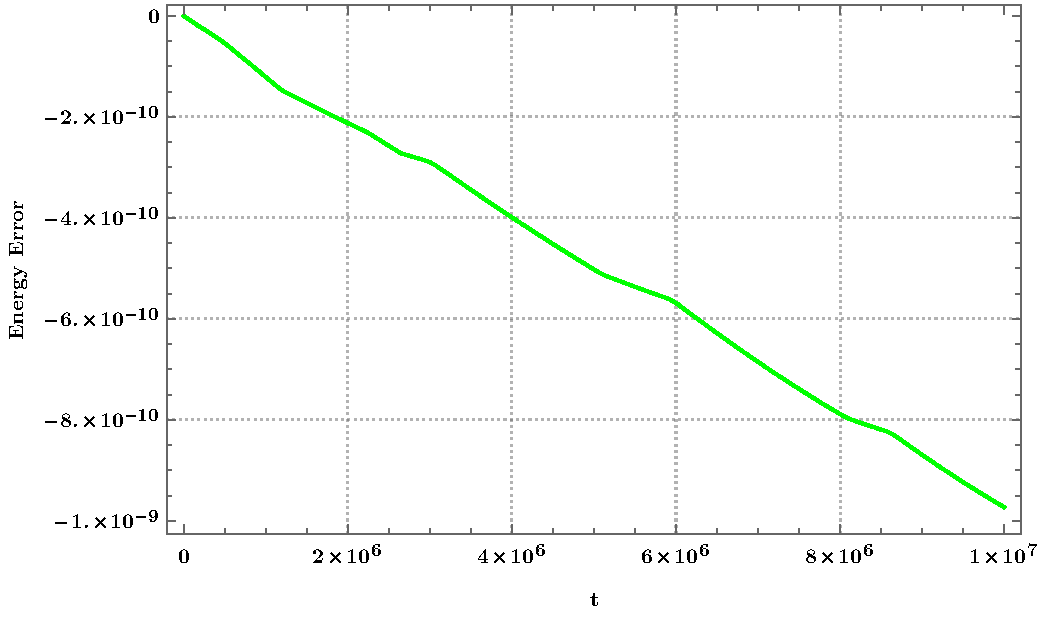
\includegraphics[width=.4\textwidth]{Fig1}}
&
\subfloat[Geratze irizpidea berria]
{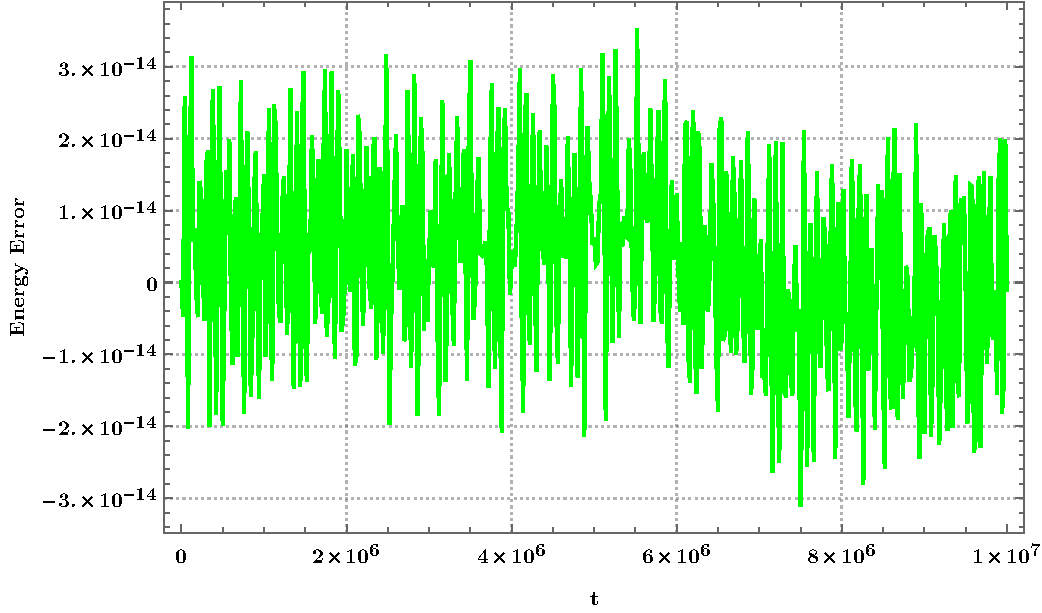
\includegraphics[width=.4\textwidth]{Fig2}}
\end{tabular}
\caption{\small Energia errore erlatiboaren eboluzioa, $h=1000/3$ urrats luzerarekin  eguzki-sistemaren kanpo-planeten problemaren integraziorako \cite{Hairer2008}. (a) Hairer-en geratze irizpidea, (b) Geratze irizpide berria}
\label{fig:OSSh2}
\end{figure}

Arazo hauei aurre egiteko, geratze irizpidea berri bat proposatuko dugu.
 Iterazioak  $k=1,2,\ldots$ jarraitzea , $ \Delta^{[k]} =0$ bete arte edo honako baldintza bi iterazio jarraietan betetzen den artean,
\begin{equation}
\label{eq:not_stopping}
\forall j \in \{1,\ldots,s d\},  \quad
\min \left(\{|\Delta_j^{[1]}|,\cdots ,|\Delta_j^{[k-1]}|\} \ /\{0\} \right) \leqslant |\Delta_j^{[k]}|.
\end{equation}

Hairer-ek, eguzki-sistemaren kanpo-planeten problemaren $h=1000/3$ eguneko urrats luzerarekin egindako integrazioa errepikatu dugu eta  geratze irizpide berriarekin, energia errorearen eboluzio zuzena dela ikus daiteke (\ref{fig:OSSh2}(b) Irudia). 


\subsubsection*{Tolerantzi testa.}

Urrats gehienetan, puntu-finkoaren iterazioak $\forall j, \ \Delta_{j}^{[k]}=0$ bete delako geratuko dira. Gainontzeko urrats gutxi horietan, zeinetan iterazioa $\exists j,  \ \Delta_{j}^{[k]} \neq 0$ izanik geratu den, orduan  urratsa onargarria den ala ez erabaki behar dugu. Iterazioa, biribiltze errorearen eraginez edo $h$ urrats luzera  behar adina txikia aukeratu ez delako, geratu daiteke.

Puntu-finkoaren iterazioak amaitzerakoan, urratsa eman aurretik erabiltzaileak definitutako tolerantzia lortu den ala ez aztertuko dugu. Horretarako, iterazioaren azken bi hurbilpenak konparatuko ditugu. Honako notazioaren laguntzarekin,
\begin{equation*}
Y_i=Y_i^{[k]}, \ \ \tilde{Y}_i=Y_i^{[k-1]}, \ \ i=1,\dots,s,
\end{equation*}  
erabiltzaileak finkatutako tolerantzia erlatiboa eta tolerantzia absolutuaren parametroen arabera ($rto_i,atol_i, i=1,\dots,d$) , \emph{distantzia normalizatua} definituko dugu,
\begin{equation*}
\max_{i=1,\dots,d} \frac{\max_{j=1,\dots,s} |Y_j^i-\tilde{Y}_j^i|}
                        {\bigg(\big((\max_{j=1,\dots,s} |Y_j^i|+\max_{j=1,\dots,s} |\tilde{Y}_j^i|)/2 \big) \ rtol_i+ atol_i \bigg)}.
\end{equation*}

Distantzi normalizatua $>1$ bada, orduan ez da lortu tolerantzia eta integrazioa amaituko dugu.
Azpimarratu behar da, tolerantzia ez dugula erabiliko puntu-finkoaren iterazio geratzeko, behin iterazioa geratu denean, urratsa onargarria den ala ez erabakitzeko baizik. Puntu-finkoaren iterazioa, konbergentzia lortu duelako edo konbergentzia arazoak izan dituelako gera daiteke. 
%Doitasun zehatzean, biribiltze errorearen eragina handia izan daiteke eta beraz, ez dugu tolerantzia estua erabiliko. Diskriminatu nahi dugu, aritmetika zehatzean konbergitu duen ala ez. Biribiltze errorea ez balitz konbergitu duen erabaki nahi dugu.

\subsection{Biribiltze errorea gutxitzeko teknikak.}

\ref{sec:4.4} ataleko koma higikorreko aritmetikaren azalpenetan, batuketa nahiz biderketa eragiketen biribiltze errore zehatza, modu errazean kalkulatu daitekeela ikusi genuen. Eragiketa hauen biribiltze erroreak, ondorengo konputazioetan erabiliko ditugu, soluzioaren doitasuna hobetzeko.

Batura errekurtsiboen konputazioen doitasuna hobetzeko teknikari \emph{batura konpensatua} esaten zaio (\ref{alg:KahanBK}) eta zenbakizko integrazioetan erabili ohi da. Atal honetan, batetik IRK metodoetan batura konpensatuaren aplikazio estandarra hobetzeko proposamena azalduko dugu. Beste aldetik, IRK metodoaren gure  inplementazioan biribiltze errorearen beste jatorri nagusiak (biderketa eta batuketa bat) modu finagoan kalkulatzea proposatuko dugu.    


\subsubsection*{Batura konpensatua.}

Zenbakizko soluzioa, $y_n \approx y(t+hn) \in \R^{d}, \ n=1,2,\dots$, bi bektoreen batura gisa, $ \ \tilde{y}_n+e_n \in \F^{d}$ lortuko dugu. Hasierako balioa $y_0 \in \R^{d}$, \ $\tilde{y}_0+e_0$ batura moduan adieraziko dugu, non $\tilde{y}_0=fl(y_0)$~ eta $e_0=fl(y_n-\tilde{y}_0)$ diren. 

Hori dela eta, IRK metodoaren inplizituki $Y_{n,i}$ atalak askatzeko ekuazioetan, $\tilde {y}_n$ balioa erabili ordez, ($\tilde{y}_n \oplus e_{n}$) espresioa erabiltzea proposatuko dugu, 
\begin{equation}
\label{eq:eqbk}
L_{n,i}^{[k]}=hb_if(Y_{n,i}^{[k-1]}), \ \ \ Y_{n,i}^{[k]}=\tilde{y}_n \oplus \big(e_{n} \oplus \sum\limits_{j=1}^{s} \mu_{ij} L_{n,j}^{[k]}\big).
\end{equation}

Aldaketa honekin, lortutako zenbakizko soluzioaren doitasuna, batura konpensatu estandarrarekin baino zerbait hobea izatea espero dugu. 

\subsubsection*{Urratsaren konputazioa.}

$\tilde{y}_{n+1}, e_{n+1} \in \mathbb{F}^d$, non $\tilde{y}_{n+1}+e_{n+1}\approx y(t_{n+1})$ den, era honetan kalkulatuko dugu:

\begin{enumerate}
\item Biderketaren biribiltze errorea.

%\begin{equation*}
%y_{n+1}=y_n+ \sum_{i=1}^{s}hb_i \ f(Y_{n,i}) 
%\end{equation*}
$hb_i f(Y_{n,i})$ biderketaren biribiltze errorea kalkulatu eta $e_{n}$ gaiari gehituko diogu. Biderketaren biribiltze errorea jasotzeko,  \emph{FMA} eragiketan oinarritutako teknika (\ref{alg:2MultFMA} algoritmoa) aplikatuko dugu. 
\begin{align*}
&E_{n,i}=hb_i \ f(Y^{[k-1]}_{n,i}) - L^{[k]}_{n,i} \ \ , \ \ i=1,\dots,s,\\
&\delta_{n}={e}_{n} + \sum\limits_{j=1}^{s}E_{n,j}.
\end{align*}


\item Batura konpensatua.

Azkenik, batura konpensatua (\ref{eq:batsd}) aplikatuko dugu,
\begin{equation}
\label{eq:bkLn}
(\tilde y_{n+1}, e_{n+1}) = S_{s,d}(\tilde y_n, \delta_n, L_{n,1}^{[k]}, \dots,L_{n,s}^{[k]}).
\end{equation}

\begin{algorithm}[H]
  \SetAlgoLined\DontPrintSemicolon
  \SetKwFunction{algo}{algo}\SetKwFunction{BaturaKonpensatua}{BaturaKonpensatua}
  \SetKwProg{myalg}{Algorithm}{}{}
  \SetKwProg{myproc}{Function}{}{}
  \myproc{\BaturaKonpensatua {$\tilde y_n$,\ $\delta_n$,\ $L_{n,1}^{[k]}, \dots,L_{n,s}^{[k]}$}}{
     \BlankLine
     $s_0=\tilde y_n$\;
     $ee=\delta_n$\;
     \For{$i\leftarrow 1$ \KwTo ($s$)}
      {
        $s_1=s_0$\;
        $\text{inc}= L_{n,i}^{[k]} +ee$\;
        $s_0=s_1+\text{inc}$\;
        $ee=(s_1 - s_0)+ \text{inc}$\;   
      }
     $\tilde y_{n+1}=s_0$\;
     $e_{n+1}=ee$\;    
    \KwRet ($\tilde y_{n+1}$,$e_{n+1}$) \;}
  \caption{BaturaKonpensatua}
\end{algorithm} 

\end{enumerate}


\subsection{Biribiltze errorearen estimazioa.}
\label{ss:634}

Zenbakizko soluzioaren $\tilde{y}_n+e_n \approx y(t_n) \ n=1,2,\dots$, biribiltze errorearen estimazioa, doitasun txikiko  bigarren zenbakizko integrazio baten soluzioaren $\hat{y}_n+\hat{e}_n \approx y(t_n)$ diferentzia gisa kalkulatuko dugu.  Jarraian, zehaztapenak emango ditugu.

$r\geqslant0$ zenbaki osoa, eta $x \in \mathbb{F}$ ($m$-biteko doitasuneko koma-higikorreko zenbakia) izanik, honako funtzioa definituko dugu,

\begin{algorithm}[H]
  \SetAlgoLined\DontPrintSemicolon
  \SetKwFunction{algo}{algo}\SetKwFunction{flr}{flr}
  \SetKwProg{myalg}{Algorithm}{}{}
  \SetKwProg{myproc}{Function}{}{}
  \myproc{\flr {x,r}}{
    \BlankLine
    $res=(2^r x + x)- 2^r x$\;
    \KwRet res \;}
  \caption{flr}
\end{algorithm} 

Funtzio honek, $(m-r)$-biteko doitasuneko koma-higikorreko zenbakia itzultzen du, edo beste modu batera esanda, $x \in \mathbb{F}$, $m$-biteko koma-higikorreko zenbakiaren azken $r$ bitak zeroan jartzen dituen funtzioa da.

Bigarren zenbakizko soluzio $(\hat{y}_n+\hat{e}_{n})$, $r$ ($r<m$) balio bat finkatuta eta inplementazioaren kalkulua (\ref{eq:bkLn}) beste era honetan egingo dugu,
\begin{equation*}
\label{eq:bkLn2}
(\hat y_{n+1}, e_{n+1}) = S_{s,d}(\hat y_n, \hat{\delta}_n, flr(L_{n,1}^{[k]},r), \dots,flr(L_{n,s}^{[k]},r)).
\end{equation*}

Zenbakizko integrazioaren biribiltze errorearen estimazioa, soluzio nagusiaren $(y_n+e_{n})$ eta $r$  balio txiki baterako (esaterako $r=3$) kalkulatutako bigarren zenbakizko soluzioaren $(\hat{y}_n+\hat{e}_{n})$ arteko diferentziaren norma bezala kalkulatuko dugu. 
\begin{equation}
estimazioa_n^i=\|(y_n^i+e_n^i)-(\hat{y}_n^i+\hat{e}_{n}^i)\|_2, \ \ i=1,\dots,d.
\end{equation}

Gure algoritmoan estimazioa lortzeko, bi integrazioak sekuentzialki modu eraginkorrean kalkulatuko ditugu. Urrats bakoitzean, bi integrazioen $Y_i,\hat{Y}_i$ ($i=1,\dots,s$) ataletako balioak, biribiltze errorearen estimazioa handiegia ez den artean, antzekoak mantentzen dira. Ondorioz, lehen integrazioaren bukaerako $Y_i^{[k]}$ ($i=1,\dots,s$) atalen balioak, bigarren integrazioaren $\hat{Y}_i^{[0]}$ (i = 1, . . . , s) atalen hasieraketarako erabiltzen baditugu, bigarren integrazioaren iterazio kopuru txikia izango da (ikus \ref{alg:errore-estimazioa} algoritmoa).  

\begin{algorithm}[H]
  \BlankLine
  \For{$n\leftarrow 0$ \KwTo ($endstep-1$)}
  {
    \BlankLine
    $Y_n^{[0]}=G(Y_{n-1},h)$\;
    \BlankLine
    $\text{\dots lehen integrazioa \dots}$\;
	\BlankLine
    $(y_{n+1},e_{n+1})\leftarrow BaturaKonpensatua(y_n,\delta_n,L_n^{[k]})$\;      
    \BlankLine
    \BlankLine
    \eIf{$(initwithfirst)$}
    {$\hat{Y}_{n}^{[0]}=Y_{n}^{[k]}+(\hat{y}_n-y_n)$\;}
    {$\hat{Y}_{n}^{[0]}=G(\hat{Y}_{n-1},h)$\;}
    \BlankLine
    $\text{\dots bigarren integrazioa \dots}$\;
	\BlankLine
    $(\hat{y}_{n+1},\hat{e}_{n+1})\leftarrow BaturaKonpensatua(\hat{y}_n,\hat{\delta}_n,flr(\hat{L}_n^{[k]},r))$\;  
    \BlankLine
    \BlankLine
    $estimation_{n+1}=\|(y_{n+1}+e_{n+1})-(\hat{y}_{n+1}-\hat{e}_{n+1})\|_2$\;
    \BlankLine
   }
 \caption{RKG2: errore estimazioa}
 \label{alg:errore-estimazioa}
\end{algorithm}
non $G()$ interpolazio funtzioa eta $initwithfirst$ egiazko balioa duen aldagaia den, integrazioen arteko diferentzia txikian den artean.

\subsection{Algoritmoa.}

Jarraian, formulazio berriari dagokion algoritmoa laburtuko dugu (\ref{alg:IRK-Berria} algoritmoa).

\begin{algorithm}[H]
 \BlankLine
  $\tilde{y}_0=fl(y_0)$\;
  $e_0=fl(y_0-\tilde{y}_0)$\;
  \For{$n\leftarrow 0$ \KwTo ($endstep-1$)}
  {
   \BlankLine
   $k=0$\;
   \text{Hasieratu}  $Y_{n,i}^{[0]} \ \ , \ \ i=1,\dots,s $\;
   \BlankLine
   \While{ (\text{not konbergentzia})}
   {
    \BlankLine 
    $k=k+1$\;
    $F_{n,i}^{[k]}=f(Y_{n,i}^{[k-1]}) $\;
    $L_{n,i}^{[k]}=hb_i \ F_{n,i}^{[k]} $\;
    $Y_{n.i}^{[k]}=\tilde{y}_{n} + \ \big(e_n+\sum\limits_{j=1}^{s} \mu_{ij} L_{n,j}^{[k]}\big)  $\;  
    $\text{konbergentzia} \leftarrow \text{GeratzeIrizpidea}(Y^{[k]},Y^{[k-1]},\Delta_{min}) $\;
   }
   \BlankLine
   \If{($\exists j \ \text{non} \ \Delta_j^{[K]}\neq 0$)}
   {
   \If{$(NormalizeDistance(Y^{[k]},Y^{[k-1]})>1$}
   {$\text{fail convergence}$\;}
   }
   $E_{n,i} = h\,   b_i\,f_{n,i}^{[k]}-L_{n,i}^{[k]}$\;
   $\delta_{n}=e_{n}+\sum_{i=1}^{s} E_{n,i}$\;
   $(\tilde y_{n+1}, e_{n+1})\leftarrow \text{baturakonpensatua}(\tilde y_{n},\delta_{n},L_{n}^{[k]})$\;
   \BlankLine
 }
 \caption{IRK (puntu-finkoa).}
 \label{alg:IRK-Berria}
\end{algorithm}

\subsubsection*{Zenbakizko soluzioa.}  

Integrazio tartea $[t_0,t_{end}]$ eta urrats tamaina $h$ bada, emandako urrats kopurua $N=(t_{end}-t_0)/h$ izango da. Bestalde, $m$ erabiltzaileak finkatutako soluzioen frekuentzia bada, $t_i=t_0+i*(m \ h), \ i=1,\dots,N/m$ uneetarako, zenbakizko soluzioa fitxategi bitar batean idatziko dugu.

Bi integrazio mota exekutatu daitezke:
\begin{enumerate}
\item Integrazio arrunta.

Integrazioaren zenbakizko soluzioa ($y_i,e_i$)  fitxategi batean itzultzen dugu eta  lerro bakoitzaren egitura honakoa da:
\begin{align*}
& (t_i,y_i,e_i) \ \text{non} \ \ t_i \in \mathbb{R} \ \text{eta} \ y_i,e_i \in \mathbb{R}^d.\\
& y_i=(q_i,p_i) \ \text{eta} \ e_i=(eq_i,ep_i).
\end{align*}

non
\begin{equation*}
(q_i+eq_i,p_i+ep_i)\approx(q(t_i),p(t_i)), \ \ \ i=1,\dots,N/m.
\end{equation*}

\item Integrazioa errore estimazioarekin.

Integrazioaren zenbakizko soluzioa ($y_i,e_i$) eta errorearen estimazioa ($est_i$)  fitxategi batean itzultzen ditugu. Lerro bakoitzaren egitura honakoa da,
\begin{align*}
& (t_i,y_i,e_i,est_i) \ \text{non} \ \ t_i \in \mathbb{R} \ \text{eta} \ y_i,e_i,est_i \in \mathbb{R}^d.\\
&  y_i=(q_i,p_i), \ e_i=(eq_i,ep_i) \ \text{eta} \ est_i=(estq_i,estp_i).
\end{align*}

\end{enumerate}


\clearpage


\section{Zenbakizko esperimentuak.}

Atal honetan, puntu-finkoaren iterazioan oinarritutako $6$-ataletako Gauss metodoaren inplementazioarekin egindako zenbakizko esperimentuak azalduko ditugu. Esperimentu hauen konputaziorako, $64$-biteko doitasuneko IEEE koma-higikorreko aritmetika erabili dugu.

\subsection{Problemak.}

Bi Hamiltondar sistema kontsideratuko ditugu: pendulu bikoitz arruntaren eta kanpo-planeten problemak \cite{Hairer2006} \cite{Dumitru}. Integrazio guztietan, $h$ urrats luzera, trunkatze errorea biribiltze errorea baino txikiago izan dadin aukeratu dugu.

\subsubsection*{Pendulu bikoitz arrunta}
Pendulu bikoitz arruntaren Hamiltondarra eta parametroak, \ref{ss:321}~atalean definitu ditugu. Sistema Hamiltondar honetarako, hasierako bi balio kontsideratu ditugu: hurrenez hurren, izaera ez-kaotikoa (NCDP) eta kaotikoa (CDP) duten mugimenduak eragiten dituztenak. Hasierako baliodun bi problema hauek (NCDP eta CDP), energia errorearen eboluzioaren eta biribiltze errorearen estimazioaren azterketa egiteko kontsideratuko ditugu. Energia errorearen jatorria aztertzeko integrazio luzerako ordea, problema ez-kaotiko (NCDP) bakarrik kontsideratu dugu.       

\subsubsection*{Kanpo-planeten problema}
Eguzki-sistemaren kanpo-planeten eredu Newtoniarra, \ref{ss:342}~atalean azaldu dugu. Hamiltondar sistema banagarria da,
\begin{equation*}
H(q,p)= T(p)+Uq),
\end{equation*}
eta ezaguna da, puntu-finkoaren iterazio estandarraren eraginkortasuna, puntu-finkoaren bertsio partizionatuarekin (\ref{alg:rkfppart})  hobetu daitekeela  \cite{Sanz-Serna1992}. Dena den, zenbakizko esperimentuetarako, Hairer-en \cite{Hairer2008} lanean bezala, puntu-finkoaren bertsio estandarraren emaitzak erakutsi ditugu. Puntu-finkoaren bertsio partizionatua aplikatu dugunean, antzeko emaitzak lortu ditugu baina urrats bakoitzean iterazio kopuru gutxiagorekin.  


\subsection{Energia errorearen jatorria.}

Doitasun bikoitzeko inplementazioaren zenbakizko soluzioaren $\tilde{y}_n+e_n \approx y(t_n) \ (n=1,2,\cdots)$ errorea, jatorri ezberdineko erroreen konbinazioa da:
\begin{enumerate}
\item Trunkatze errorea: hasierako baliodun problemaren soluzio zehatza $y(t_n)$ ($n=1,2,3,\cdots$), (\ref{eq:irk1})-(\ref{eq:irk2}) metodoa aplikatuz  ($b_i,\mu_{ij}$ koefiziente zehatzekin) lortutako zenbakizko soluzioa $y_n$ ordezkatzerakoan eragindako errorea. 
\item Iterazio errorea: praktikan, puntu-finkoaren (\ref{alg:pf}) $K$ iterazio finitu aplikatzen da, eta (\ref{eq:irk1}) sistemaren $L_{n.i}, Y_{n,i} \ (i=1,\cdot,s)$ soluzioa, $L_{n.i}^{[K]}, Y_{n,i}^{[K]}$ hurbilpenarekin ordezkatzen da. Hurbilpen honen araberako $\bar{y}_{n+1}$ zenbakizko soluzioa kalkulatzen da,
\begin{equation*}
\bar{y}_{n+1}=y_{n}+\sum_{i=1}^{s} L_{n,i}^{[K]}.
\end{equation*}   
\item Funtzioa zehatza $f:\mathbb{R}^d \rightarrow \mathbb{R}^d$, bere doitasun bikoitzeko bertsioaz $\tilde{f}:\mathbb{F}^d \rightarrow \mathbb{F}^d$ ordezkatzerakoan, sortutako errorea.  Ordezkapen honek, bi eragin ditu: batetik, urrats gehienetan $K$ iterazio finituetan puntu-finkora iritsiko gara, zeinek  ekidin ezineko iterazio errorea sortuko duen; bestetik, $\tilde{f}$ funtzioaren konputazioan sortatutako biribiltze erroreak. 
\item IRK metodoaren koefiziente zehatzak $b_i,\mu_{ij} \in \mathbb{R}$, dagozkien doitasun bikoitzeko koefiziente $\tilde{b}_i,\tilde{\mu}_{ij} \in \mathbb{F}$ erabiltzeagatik eragindako errorea.
\item Algoritmoaren inplementazioaren eragiketa aritmetikoak ($\tilde{f}$ funtzioaren ebaluazioa egindakoaz gain), doitasun bikoitzean kalkulatzeagatik eragindako errorea.  
\end{enumerate} 

Errore jatorri hauek energian duten eragina estimatzeko, honako algoritmoak inplementatu ditugu:

\begin{enumerate}
\renewcommand{\theenumi}{\Alph{enumi}}

\item Inplementazio zehatza.

Trunkatze errorea estimatzeko, konputazio guztiak (ekuazio diferentzialaren funtzioaren ebaluazioa barne) doitasun laukoitzeko ($128$-bit) koma higikorreko aritmetikan kalkulatzen duen inplementazioa aplikatuko dugu. 

%Zenbakizko integrazio hau, trunkatze errorea estimatzeko eta errore globala kalkulatzeko erreferentzi gisa (soluzio zehatza) kontsideratuko dugu. 

\item Inplementazio superideala.

Zenbakizko integrazio hau, iterazio errorea estimatzeko erabiliko dugu. Konputazio guztia doitasun laukoitzean egindako inplementazioa baina geratze irizpidea, doitasun bikoitzean neurtuko dugu,
\begin{equation*}
\Delta^{[k]}=|\text{double}(Y^{[k]})-\text{double}(Y^{[k-1]})|.
\end{equation*}

\item Inplementazio ideala.

Ekuazio diferentzialaren eskuin aldeko funtzioaren ebaluazioa izan ezik, beste eragiketa guztiak doitasun laukoitzean kalkulatzen dituen inplementazioa da. Ekuazio diferentziala doitasun bikoitzean kalkulatzeak, eragiten duen errorea neurtzeko erabiliko dugu eta integrazio hau hobetu ezin daitekeen integrazioa kontsideratuko dugu.  

\item Inplementazio sasi-ideala.

Doitasun bikoitzeko koefizienteak ($\tilde{\mu}_{ij},\tilde{b}_i \in \mathbb{F}$) erabiltzeak eragiten duen errorea neurtzeko integrazioa da. Konputazio guztia doitasun laukoitzean kalkulatzen da baina doitasun bikoitzeko koefizienteen balioak erabiliz (hauei doitasun bikoitzeko koefiziente koadrifikatuak esaten diogu). 

\end{enumerate}


Hasierako baliodun problema bakoitzaren, goian azaldutako A--D inplementazio bakoitzari dagokion energia errorearen eboluzioa erakutsi dugu (\ref{fig:SourceError} irudia). Aukeratutako $h$ urrats luzerarentzat, trunkatze errorea biribiltze errorearen azpitik dagoela baieztatu dugu.
Metodoaren doitasun bikoitzeko koefizienteak ($\tilde{b}_i, \tilde{\mu}_{ij}\in \mathbb{F}$) erabiltzeak, ez du eraginik biribiltze errorearen garapenean.  Iterazio errorea, biribiltze errorearen oso antzeko da, eta energia errorearen drift lineala eragitea espero daiteke. 

\begin{figure}[h!]
\centering
\begin{tabular}{c c}
\subfloat[NCDP ($h=2^{-7}$)]
{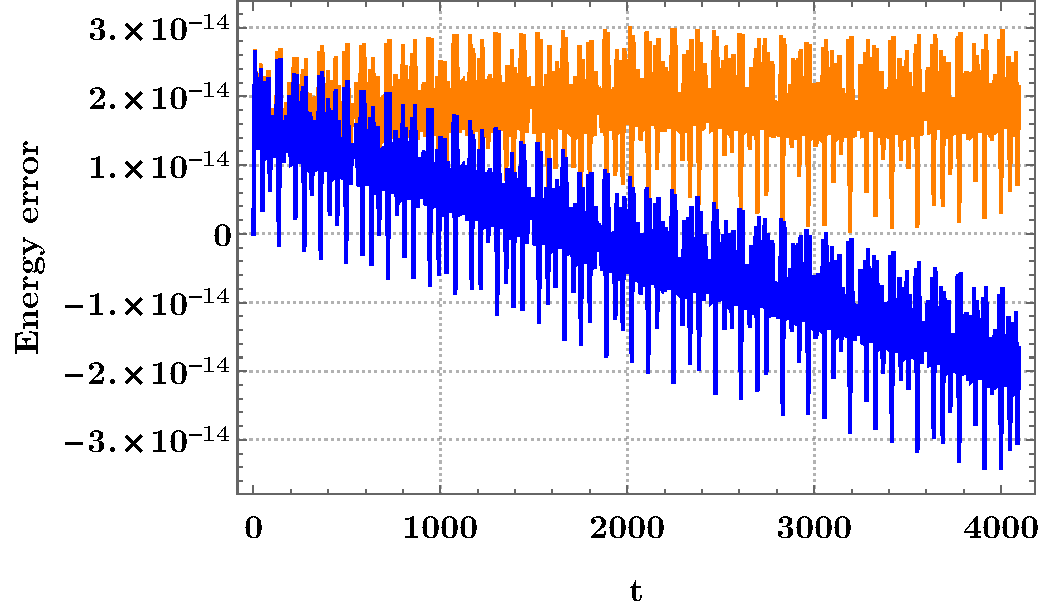
\includegraphics[width=.600\textwidth]{Fig4}}\\
\subfloat[OSS ($h=500/3$)]
{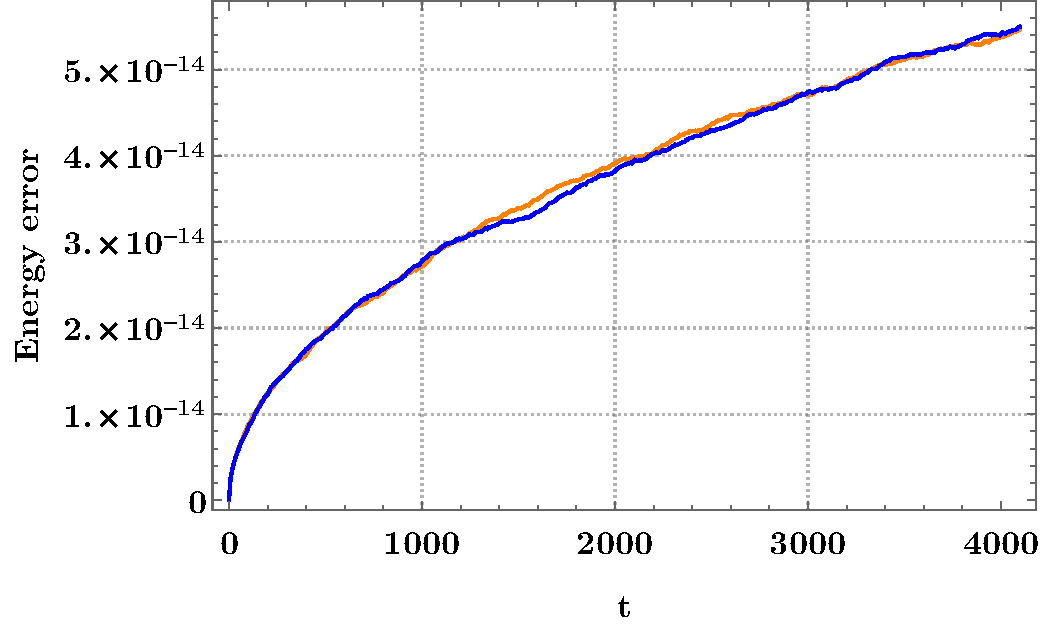
\includegraphics[width=.600\textwidth]{Fig5}}
\end{tabular}
\caption{\small Algoritmo inplementazio ezberdinetarako, energiaren errore erlatiboa eskala logaritmikoan irudikatu dugu: A-algoritmoa trunkatze errorearen estimazioa (gorriz), B-algoritmoa  iterazio errorearen estimazioa (berdez), C-algoritmoa doitasun bikoitzean $\tilde{f}$ funtzioaren ebaluazioaren eraginaren estimazioa (beltzez), doitasun bikoitzeko $\tilde{b}_i, \tilde{\mu}_{ij} \in \mathbb{F}$ koefizienteak aplikatzearen estimazioa (urdinez). Hasierako baliodun problema bakoitzarentzat, irudi bana egin dugu: pendulu bikoitzaren problema ez-kaotikoa (a) eta kanpo-planeten problema (b).}    
\label{fig:SourceError}
\end{figure}

\subsection{Errore azterketa estatistikoa.}

Biribiltze erroreak eragiten duen zenbakizko erroreen azterketa fidagarriagoa egiteko, analisi estatistikoa aplikatu dugu (Hairer-en \cite{Hairer2008} lanean bezala). Problema bakoitzarentzat, hasierako balioaren osagai bakoitza ausaz perturbatutako ($\mathcal{O}(10^{-6})$ tamainako errore erlatiboarekin) $P=1000$ integrazio exekutatu ditugu eta emaitza hauen guztien batezbestekoan oinarritu gara, biribiltze errorearen azterketa zehatzagoa egiteko.    

Puntu-finkoaren iterazioan oinarritutako $6$-ataletako Gauss kolokazio metodoaren hiru inplementazio konparatu ditugu:
\begin{enumerate}
\item Inplementazio ideala: ekuazio diferentzialaren eskuin aldeko funtzioaren ebaluazioa izan ezik, beste eragiketa guztiak doitasun laukoitzean ($128$-bit) kalkulatzen dituen inplementazioa da. Inplementazio hau FPIEA (fixed point iteration with exact arithmetic) izendatuko dugu.

\item Doitasun bikoitzeko gure inplementazioa berria. Inplementazioa hau, DP izendatu dugu.

\item Hairer-ek proposatutako inplementazioa ~\cite{Hairer2008}. Zenbakizko esperimentuetarako, Hairer-en IRK metodoaren Fortran kodea exekutatu dugu (\href{http://www.unige.ch/~hairer/preprints.html}{Kodea}).     

\end{enumerate}

Batetik, DP inplementazioaren biribiltze errorearen garapena, FPIEA  inplementazioaren (aritmetika zehatza) errorearekiko kualitatiboki antzekoa den eta magnitudean gertu dagoen ziurtatu nahi dugu. Bestalde, DP inplementazioa, Hairer-en inplementazioarekin konparatu nahi dugu.

Aipatutako hiru inplementazioetarako, puntu-finkoa lortu den urratsen portzentaia eta iterazio batezbestekoa laburtu ditugu (\ref{tab:fperr}~taula). 

\begin{table}
\caption[ Urratsen puntu-fikoaren iterazio portzentaia eta iterazio batezbestekoa.] 
{\small{ Puntu-finkoa lortu den urratsen portzentaia eta iterazio batezbestekoa, pendulu bikoitzaren problema ez-kaotikorako (NCDP), pendulu bikoitzaren problema kaotikorako (CDP), eta kanpo-planeten problemarako (OSS). Zutabetan, hiru inplementazioa konparatu ditugu: FPIEA (ideala), DP (doitasun bikoitza) eta Hairer-en kodea.}}
\label{tab:fperr}       % Give a unique label
\centering
%\resizebox{\textwidth}{!}
{%
\begin{tabular}{ l c c c c c c } 
 \hline
                 &  \multicolumn{2}{c}{FPIEA}  & \multicolumn{2}{c}{DP} & \multicolumn{2}{c}{Hairer} \\
                 &     $\%$        &  $\#$        &      $\%$           &   $\#$      &    $\%$       &  $\#$      \\
 \hline
 NCDP            & $98.7$    & $9.5$   & $98.8$     & $8.6$   &  $98.5$ & $8.6$  \\ 
 CDP             & $98.9$    & $9.5$   & $98.9$     & $8.6$   &  $98.4$ & $8.6$  \\ 
 OSS             & $97.4$    & $15.2$  & $97.4$     & $14.2$  &  $87.5$ & $14.1$ \\ 
   \hline
 \end{tabular}}
 \end{table}


\subsubsection*{Energia diferentzien banaketa.}

\begin{figure}[h!]
\centering
\begin{tabular}{c c}
\subfloat[\small {NCDP}]
{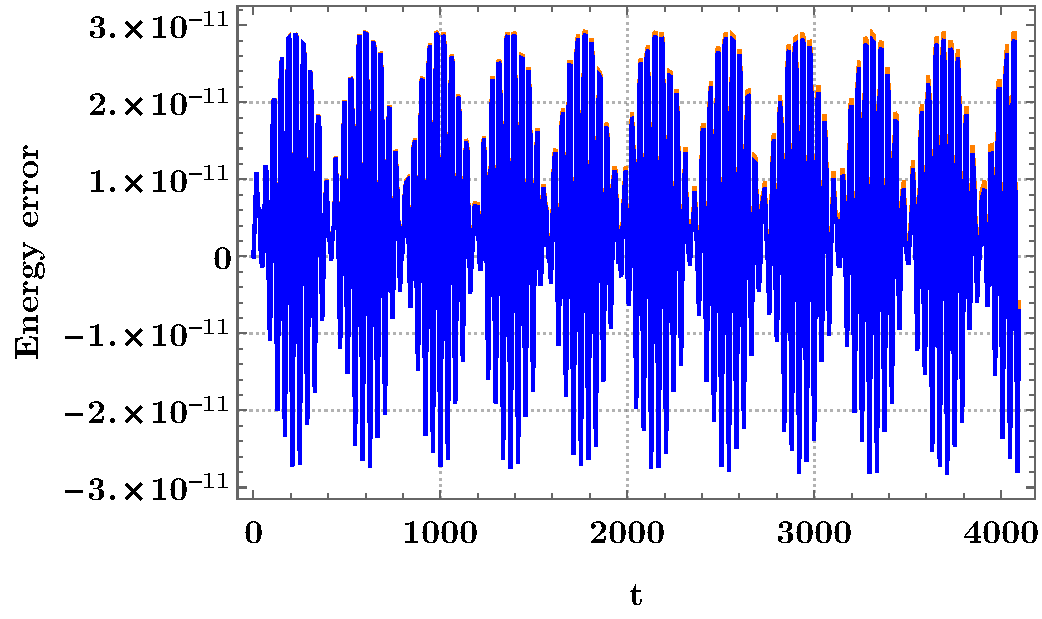
\includegraphics[width=.4\textwidth]{Fig6}} %Fig6
&
\subfloat[OSS]
{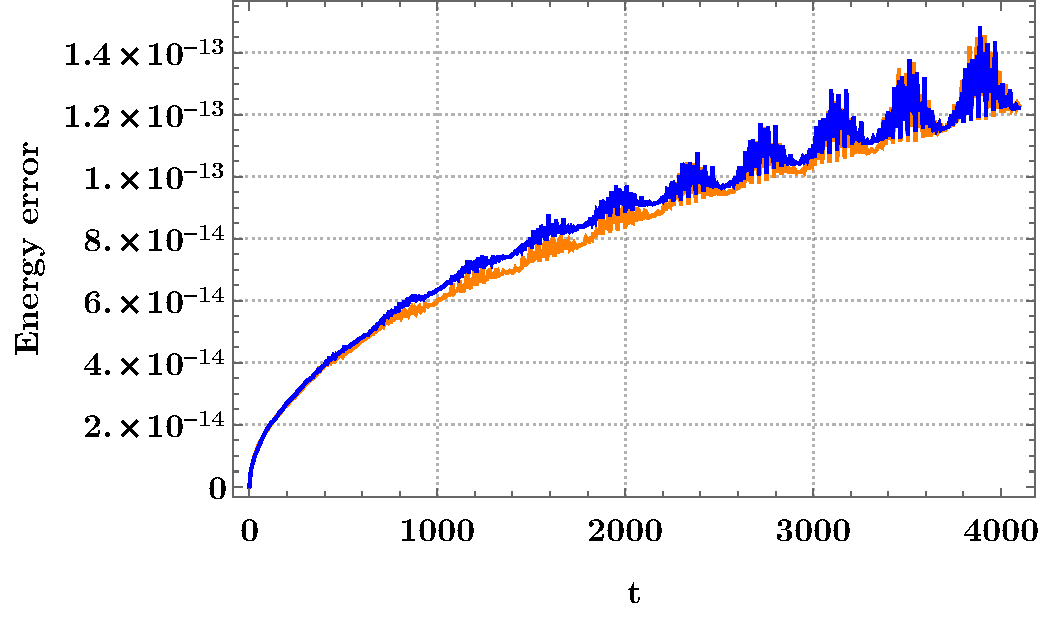
\includegraphics[width=.4\textwidth]{Fig7}} %Fig7
\\
 ($\mu=5.3\times 10^{-19}$, \ $\sigma=1.5\times 10^{-17}$) &
 ($\mu=-1.9\times 10^{-19}$, \ $\sigma=3.5\times 10^{-18}$) 
 \end{tabular}
\caption{ \small DP inplementazioarekin lortutako $K P$ energia diferentzien histogramak, eta $N(\mu, \delta)$ banaketa normala, pendulu bikoitzaren problema ez-kaotikoarentzat (NCDP) eta kanpo-planeten problemarentzat (OSS). Ardatz horizontala $10^{15}$ balioarekin biderkatu dugu eta ardatz bertikalak, maiztasuna adierazten du}
\label{fig:hist}
\end{figure}


Integratzailearen inplementazioa ona bada, biribiltze erroreak eragindako energiaren errore lokala $H(y_n)-H(y_{n-1}$), ausazkoa izatea espero da. Hortaz, zenbakizko soluzioa $m$ urratsero jasotzen dugula jakinik, energi diferentzia $H(y_{km})-H(y_{km-m})$ ausazkoa izatea espero da, $\mu$ batezbestekoa ($\mu=0$ idealki) eta $\sigma$ desbideratzea duen banaketa Gausiarrarekin. Ondorioz, metatutako energia diferentzia,
\begin{equation*}
H(y_{km})-H(y_0),
\end{equation*} 
$t_{mk}=t_0+kmh$ uneetarako, $k^{1/2} \sigma=(t_{mk}/(mh))^{1/2} \sigma$ desbideratze estandarra duen ausazko ibilbide Gaussiar bat (\emph{random walk}) jarraituko du. Honi, konputazio zientzian ~\cite{Grazier2005} Brouwer legea deritzote, Brouwer-ek ~\cite{Brouwer1937} Kepler problemarentzat  egin zuen zenbakizko integrazioaren birbiltze errorearen azterketa gogoratuz.

Ideia hau jarraituz, doitasun bikoitzeko (DP) inplementazioan, $m$ urrats arteko energiaren diferentziak,
\begin{equation*}
\frac{H(y_{km})-H(y_{km-m})}{H(y_0)},
\end{equation*} 
banaketa Gaussiarra dagokion aztertuko dugu.   

Integrazio tartea $[t_0, t_{end}]$  eta $P$ perturbatutako hasierako balioen kopurua bada, $KP$ energia diferentzien balio ditugu,
non $K=(t_{end}-t_0)/(mh)$ den. DP inplementazioarekin lortutako $KP$ energia diferentzien histograma eta $N(\mu,\sigma)$ banaketa normala irudikatu ditugu (non $\mu$ eta $\sigma$, balioei dagokien batezbestekoa eta desbideratze tipikoak diren). \ref{fig:hist} irudian, pendulu bikoitzaren problema ez-kaotikoari (NCDP), eta kanpo-planeten problemari (OSS) dagozkien histogramak, $N(\mu,\sigma)$ banaketa normalari oso ondo egokitzen zaiela ikus daiteke.


\subsubsection*{Errore batezbestekoaren eta desbideratze estandarraren eboluzioa}


\ref{fig:Htt}~irudian, FPIEA, DP eta Hairer-en inplementazioetarako, NCDP eta OSS problemen integrazioen energia errorearen batezbestekoa eta desbideratze estandarra irudikatu ditugu.

\begin{figure}[h!]
\centering
\begin{tabular}{c c}
\subfloat[NCDP: energi errorea]
{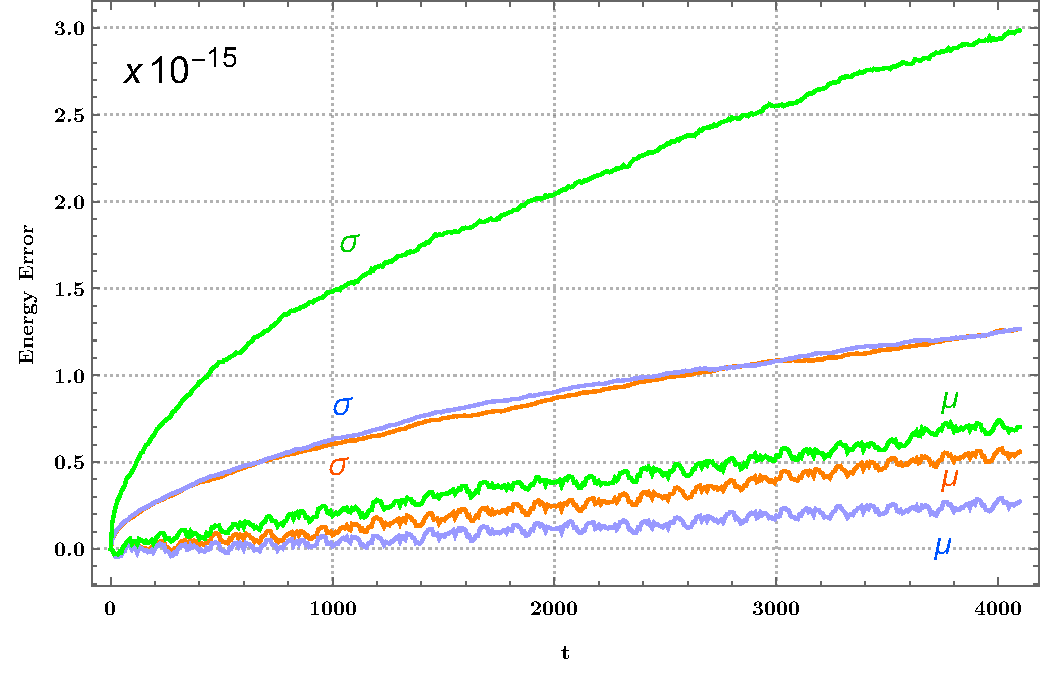
\includegraphics[width=.4\textwidth]{Fig8}}
&
\subfloat[NCDP: energi errorearen batezbestekoa]
{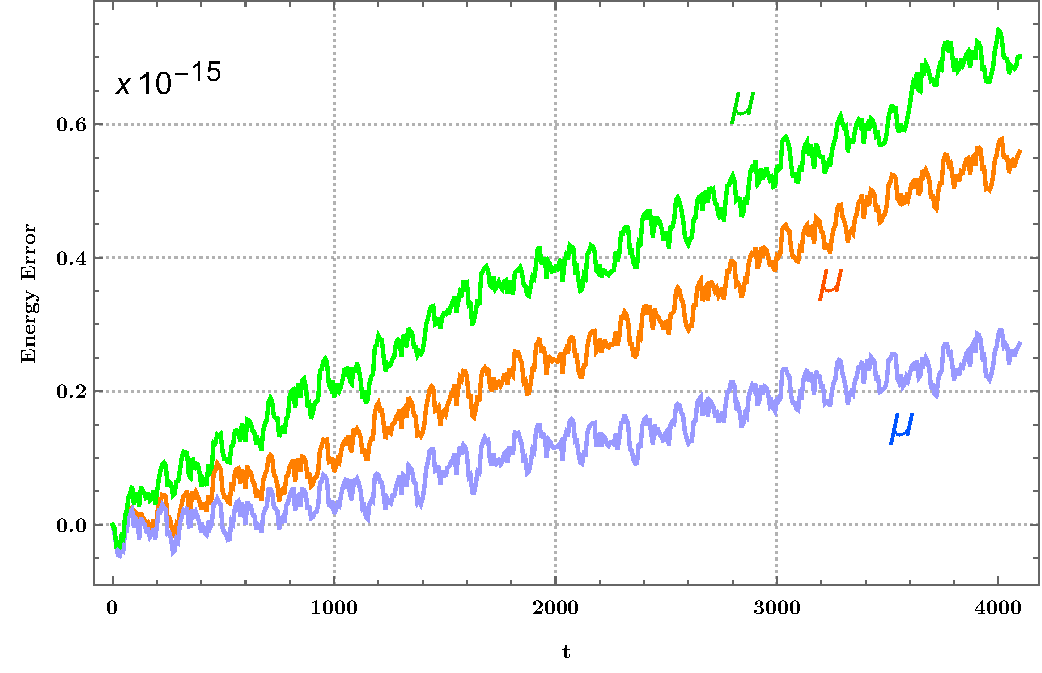
\includegraphics[width=.4\textwidth]{Fig9}}
\\
\subfloat[OSS: energi errorea]
{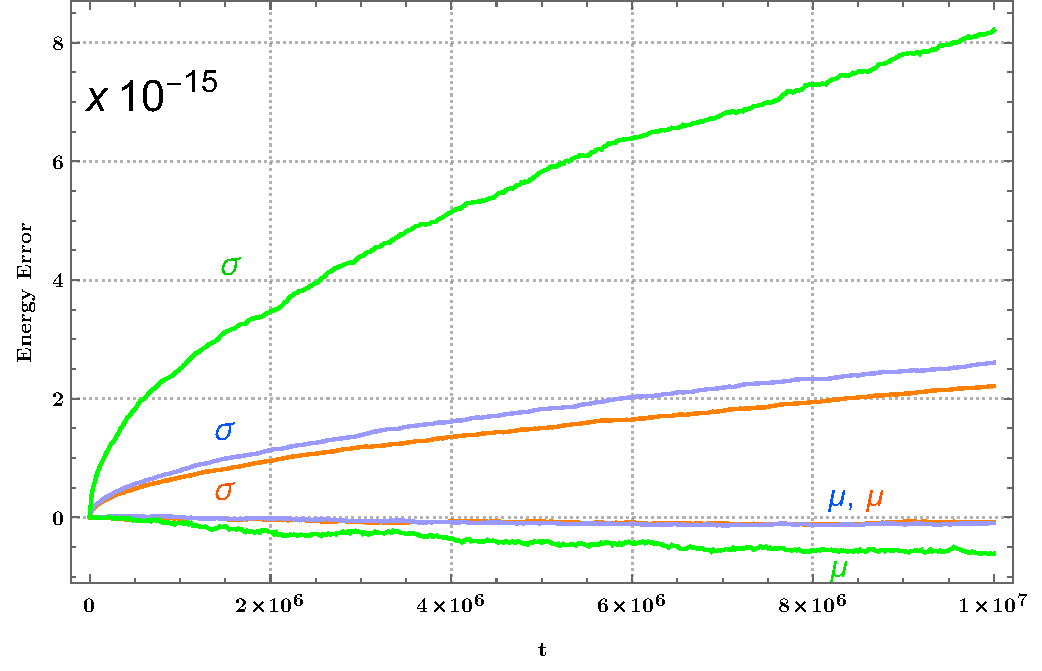
\includegraphics[width=.4\textwidth]{Fig10}}
&
\subfloat[OSS: energi errorearen batezbestekoa]
{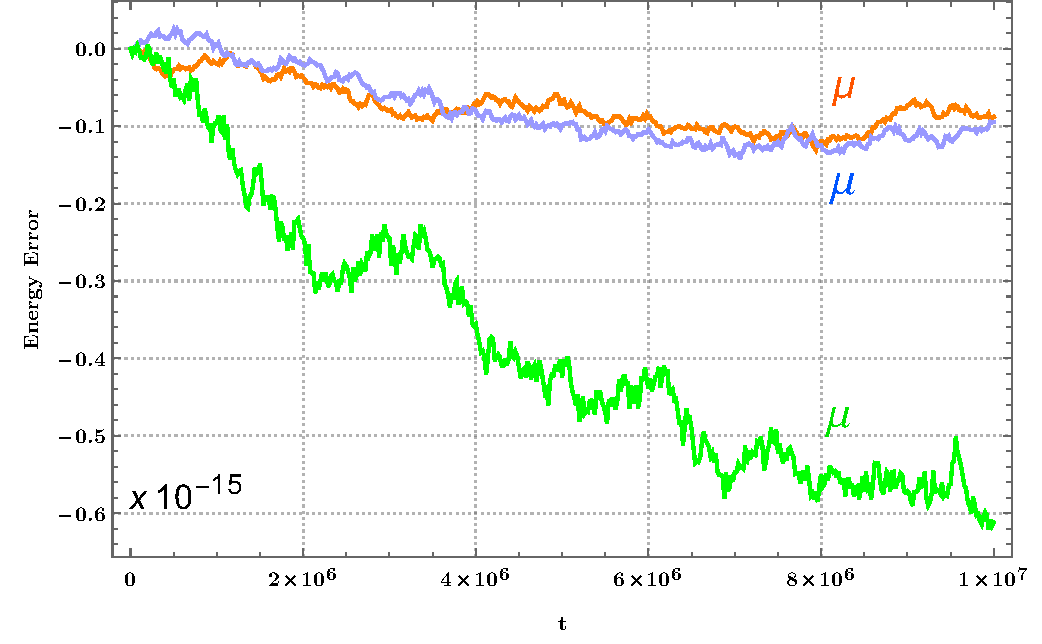
\includegraphics[width=.4\textwidth]{Fig11}}
\end{tabular}
\caption{\small Energi errorearen batezbestekoa ($\mu$) and desbideratze estandarra ($\sigma$) (ezkerrean) eta energi errorearen batezbestekoaren zehaztapena (eskubian), DP inplementazioarentzat (urdinez), FPIEA inplementazioarentzat (laranjaz), eta Hairer-en inplementazioarentzat (berdez). Pendulu bikoitzaren problema ez-kaotikoa (a,b) eta kanpo-planeten problema (c,d) }
\label{fig:Htt}
\end{figure}

FPIEA, puntu-finkoaren iterazioan oinarritutako IRK inplementazio optimoena kontsideratu daiteke, $f$ funtzioari dagokion doitasun bikoitzeko $\tilde{f}$ funtzioa aplikatuko dugula suposatzen badugu. Argitu beharra dago, esperimentu hauetan FPIEA inplementazioaren geratze irizpidea DP inplementazioarena baino gogorragoa erabili dugula: iterazioa geratu dugu $\Delta^{[k]}=0$ delako edo (\ref{eq:not_stopping})~baldintza hamar iterazio jarraian bete delako. Era honetan, puntu-finkoa lortu ez den urratsetarako, iterazio errorea ekiditen saiatu gara.

\ref{fig:Htt}~irudiko zenbakizko esperimentuetan, DP inplementazioaren energi errorearen batezbesteko eta desbideratze tipikoaren eboluzioa ia optimoa da (FPIEA inplementazioarekiko gertu). 

Puntu-finkoaren iterazioan oinarritutako IRK metodoen inplementazioan, energi errorearen batezbestekoan drift lineal txiki bat (NCDP problemarentzat) ekidin ezinezkoa dela sinistuta gaude. Esperimentu hauen energi errorearen eboluzioak, \ref{fig:SourceError}~irudian erakutsitako iterazio errorea, birbiltze errorearen gertu egoteagatik egindako iruzkinarekin kontsistenteak dira.

Energia drift-a, ez da IRK metodo sinplektikoen berezko arazoa. \ref{fig:plotNewton}~irudian, Newton sinplifikatuaren iterazioan oinarritutako IRK inplementazioarekin NCDP problemaren aurreko esperimentua errepikatu dugu eta energi errorearen batezbestekoaren eboluzioan ez da drift linealik agertzen.   

\begin{figure}[h!]
\centering
\begin{tabular}{c c}
\subfloat[NCDP: energi errorea.]
{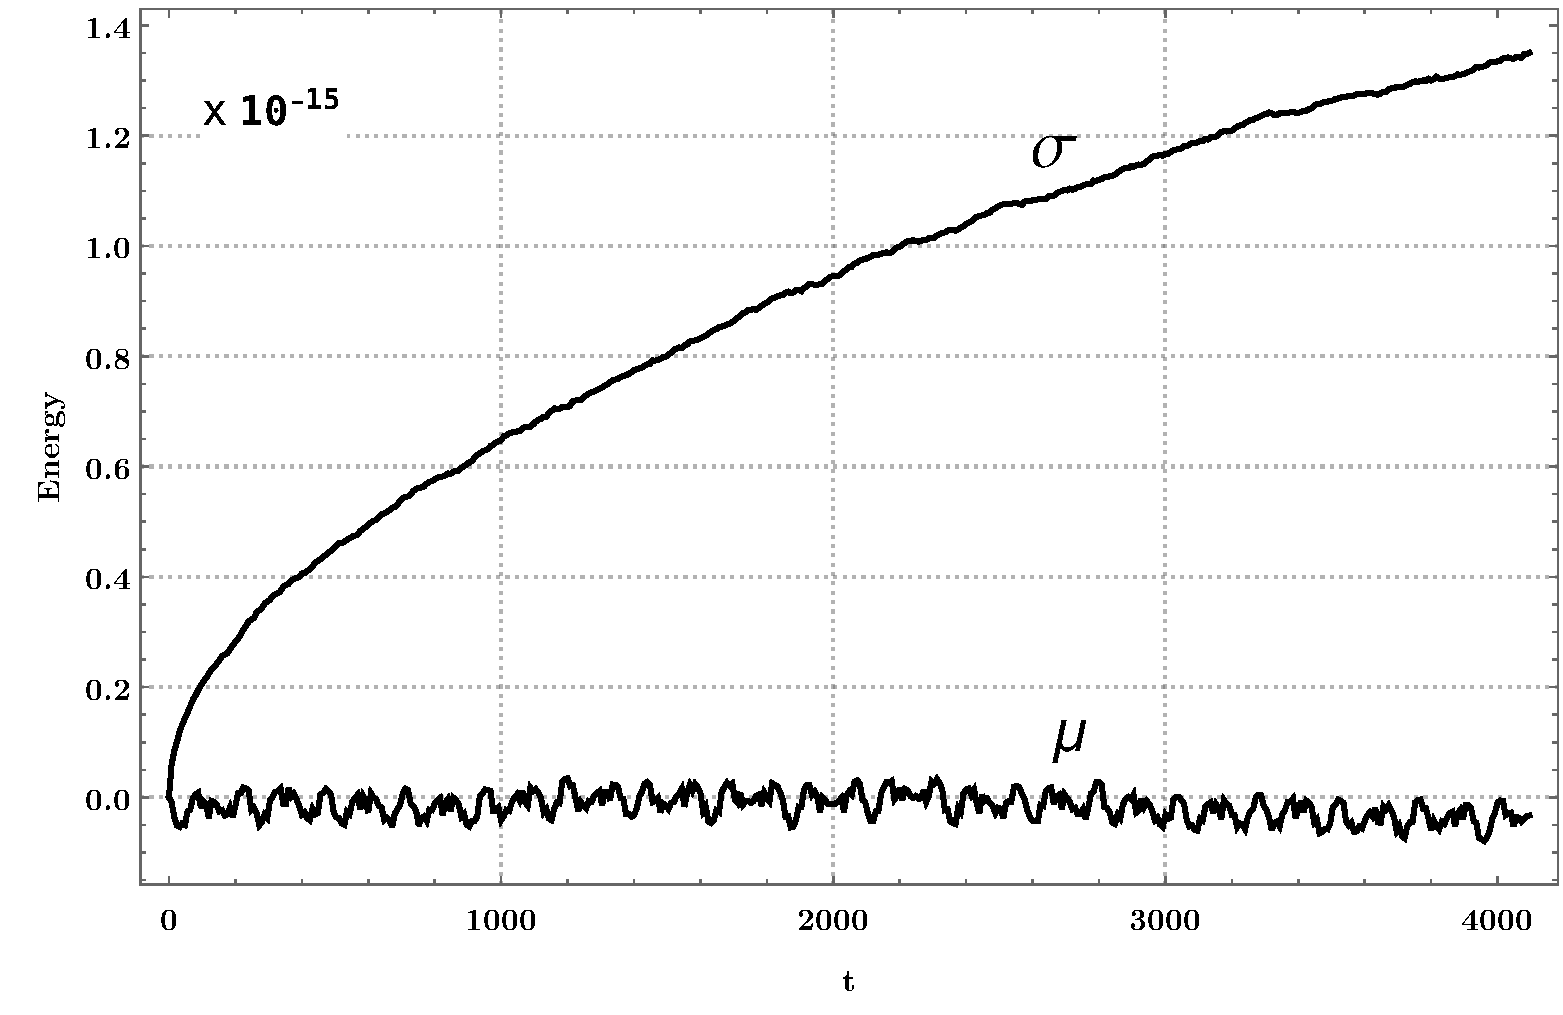
\includegraphics[width=.4\textwidth]{Fig12}}
&
\subfloat[NCDP: energi errorearen batazbestekoa.]
{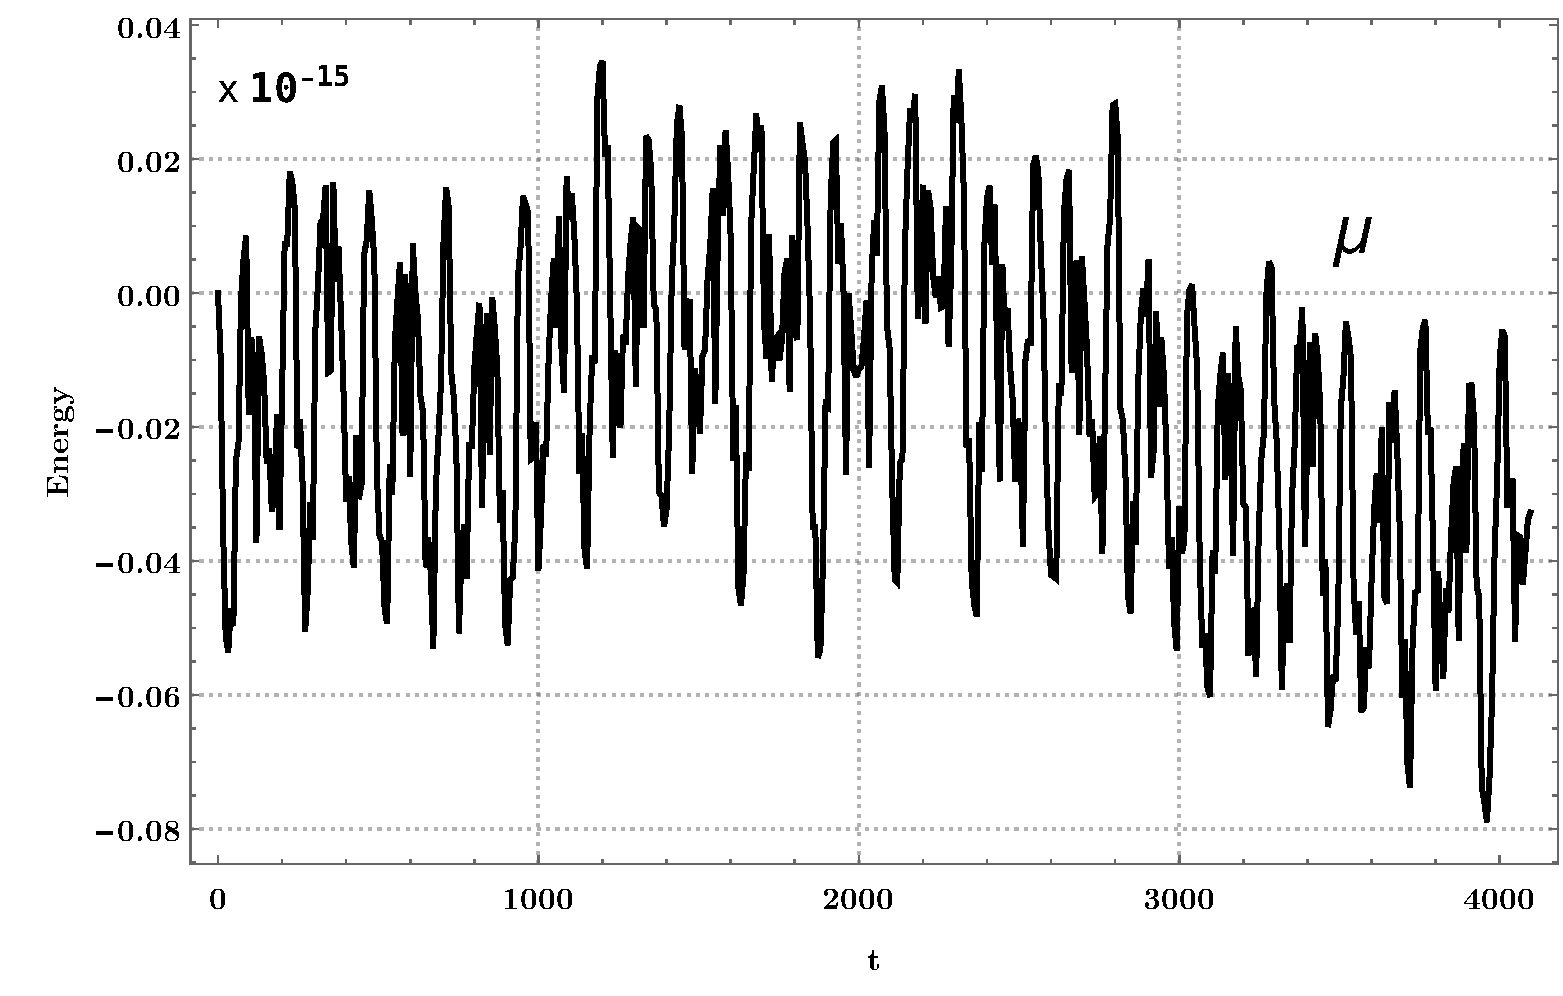
\includegraphics[width=.4\textwidth]{Fig13}}
\end{tabular}
\caption{\small Energi errorearen batezbestekoa ($\mu$) eta desbideratze estandarra ($\sigma$), Newton sinplifikatuaren iterazioan oinarritutako IRK inplementazioarekin}
\label{fig:plotNewton}
\end{figure}

Zenbakizko esperimentuen atala amaitzeko, \ref{fig:plot4}~irudian, FPIEA, DP eta Hairer-en inplementazioen integrazioen kokapen errorearen eboluzioa (batezbestekoa eta desbideratze estandarra) erakutsi ditugu. Emaitza hauek, DP inplementazioa, puntu-finkoaren iterazioan oinarritutako inplementazio optimoaren oso gertu dagoenaren ideia indartu egiten dute.


\begin{figure}[h!]
\centering
\begin{tabular}{c c}
\subfloat[NCDP: kokapen errorearen batezbestekoa.]
{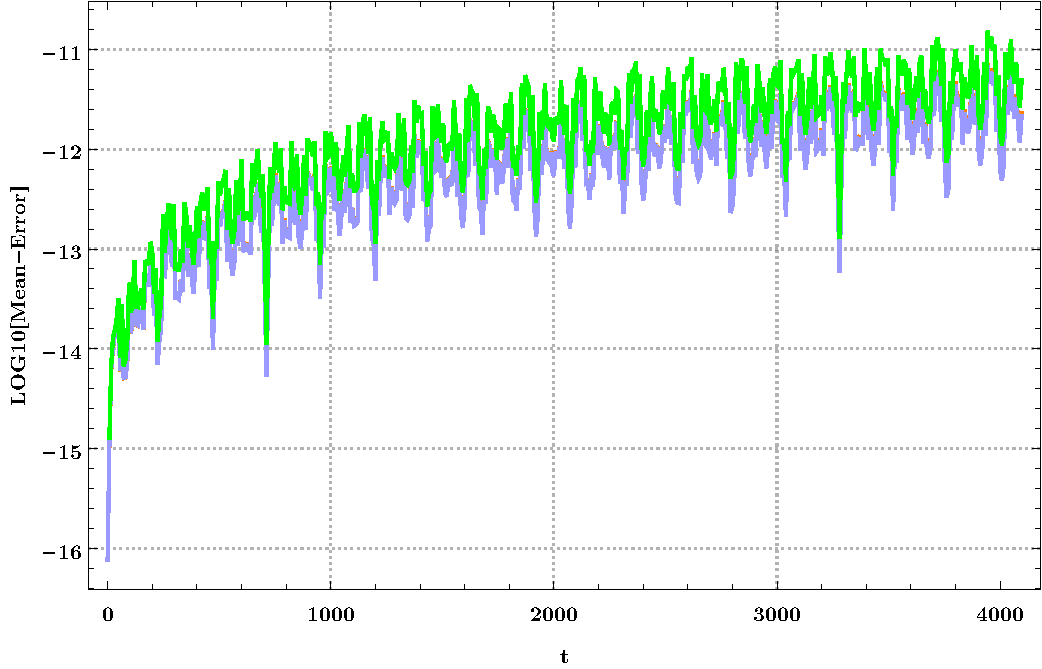
\includegraphics[width=.4\textwidth]{Fig14}}
&
\subfloat[NCDP: kokapen errorearen desbideratzea.]
{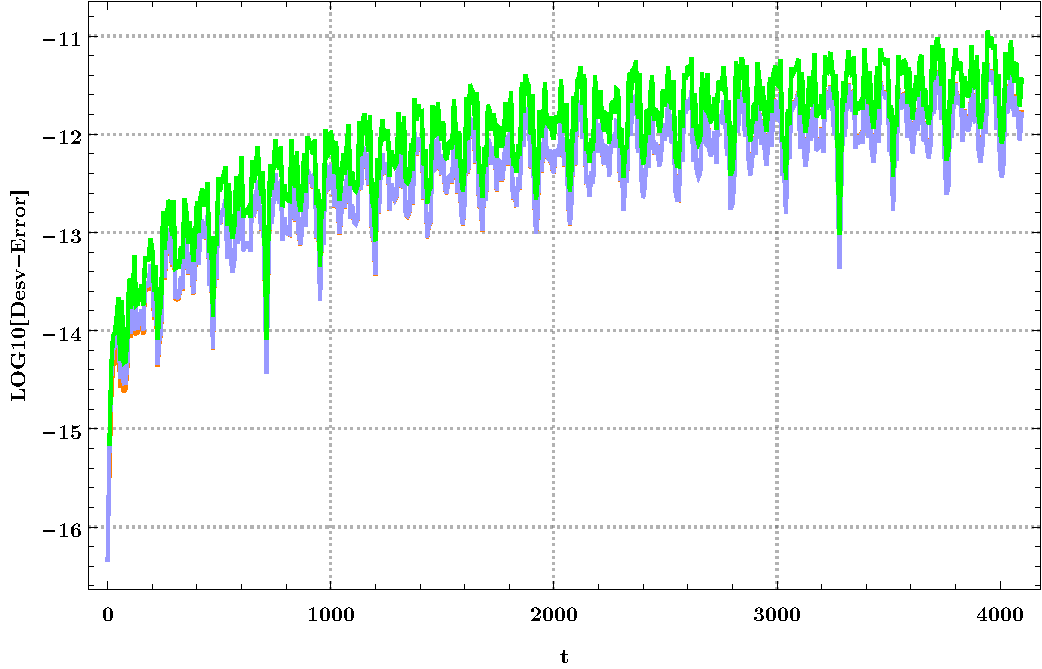
\includegraphics[width=.4\textwidth]{Fig15}}
\\
\subfloat[CDP: kokapen errorearen batezbestekoa.]
{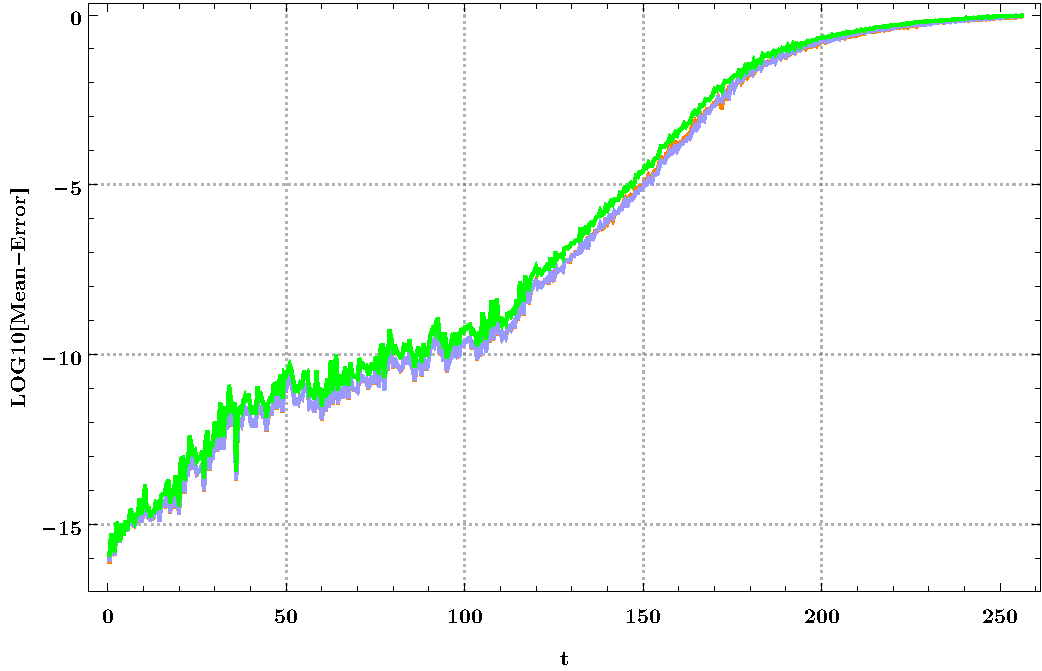
\includegraphics[width=.4\textwidth]{Fig16}}
&
\subfloat[CDP: kokapen errorearen desbideratzea.]
{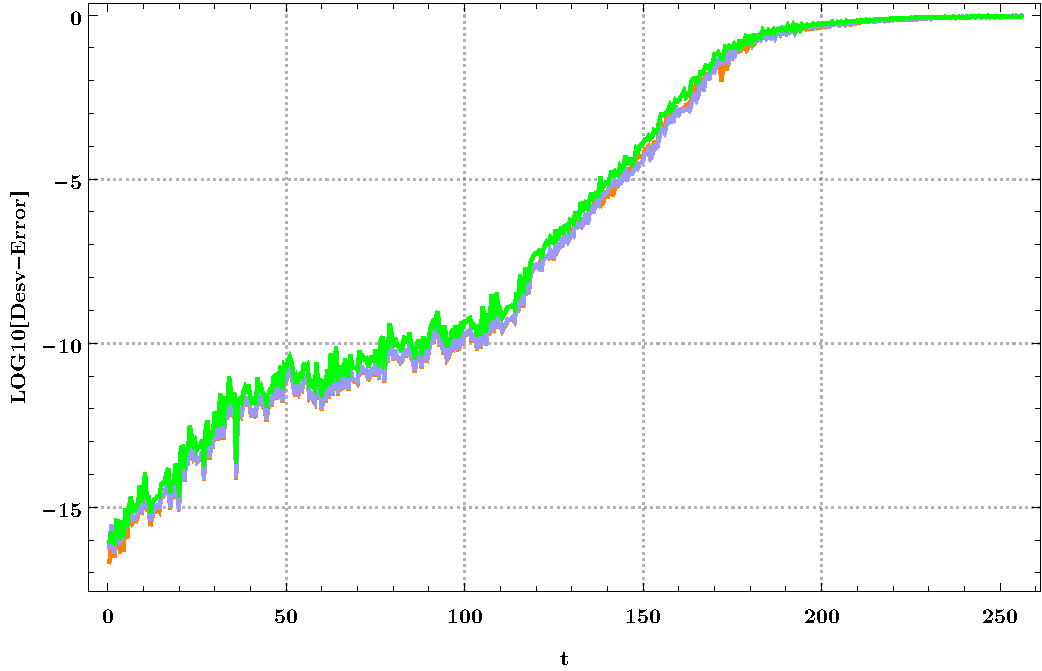
\includegraphics[width=.4\textwidth]{Fig17}}
\\
\subfloat[OSS: kokapen errorearen batezbestekoa.]
{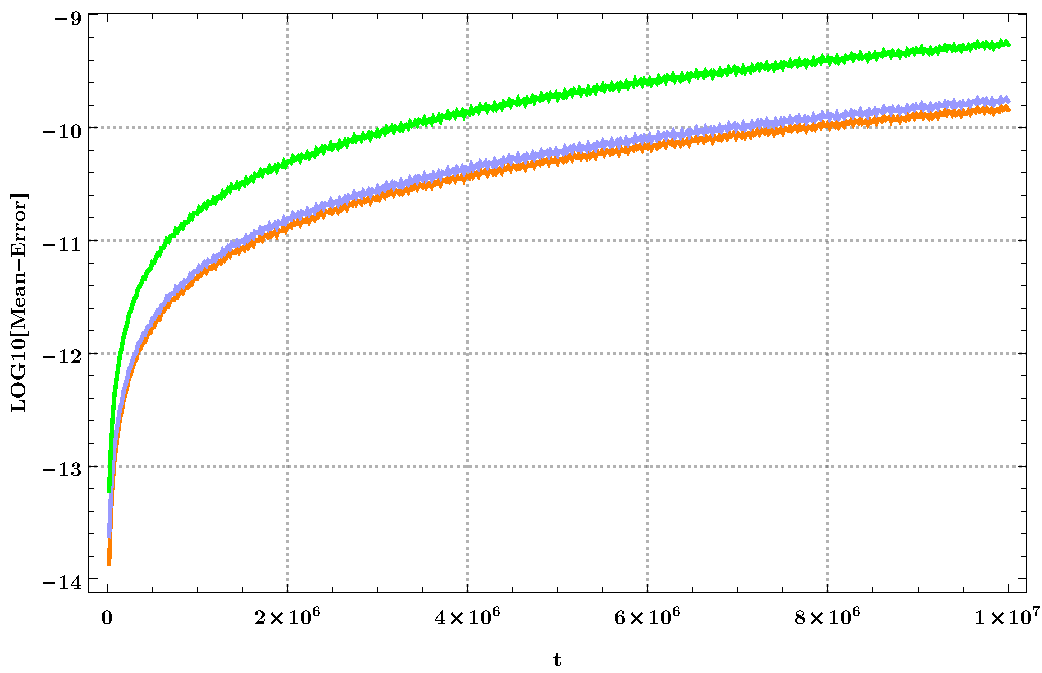
\includegraphics[width=.4\textwidth]{Fig18}}
&
\subfloat[OSS: kokapen errorearen desbideratzea.]
{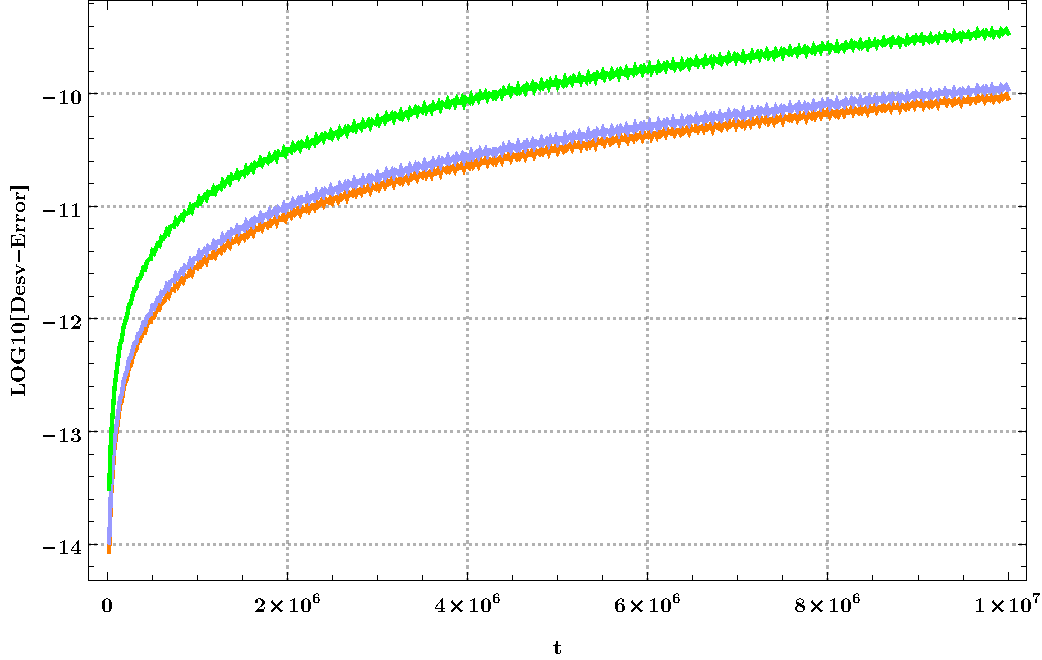
\includegraphics[width=.4\textwidth]{Fig19}}
\end{tabular}
\caption{\small Kokapen errorearen batezbestekoa (ezkerrean) eta desbideratze estandarra (eskubian), DP inplementazioarentzat (urdinez), FPIEA inplementazioarentzat (laranjaz) eta Hairer-en inplementazioarentzat (berdez): NCDP (a,b), CDP (c,d) eta OSS (e,f)}
\label{fig:plot4}
\end{figure}

\subsection{Biribiltze errorearen estimazioa}


\ref{ss:634}~atalean deskribatutako biribiltze errorearen estimazioa kalkulatzeko teknika aplikatu dugu.  \ref{fig:plot5}~irudian, hiru problemetarako (perturbatu gabeko hasierako balioa erabiliz) DP inplementazioaren integrazioaren kokapen errorea eta  kokapen errorearen estimazioa ($r=3$ aplikatuta) irudikatu ditugu. Era berean, hiru problemen hasierako balioen perturbatutako $P=1000$, DP inplementazioaren integrazioen kokapen errorearen batezbestekoa eta kokapen errorearen estimazioaren batezbestekoak konparatu ditugu. Emaitza hauek, proposatutako biribiltze errorearen estimazioa kalkulatzeko teknikaren erabilgarritasuna erakusten dutela uste dugu.  

\begin{figure}[h!]
\centering
\begin{tabular}{c c}
\subfloat[NCDP: jatorrizko hasierako balioak]
{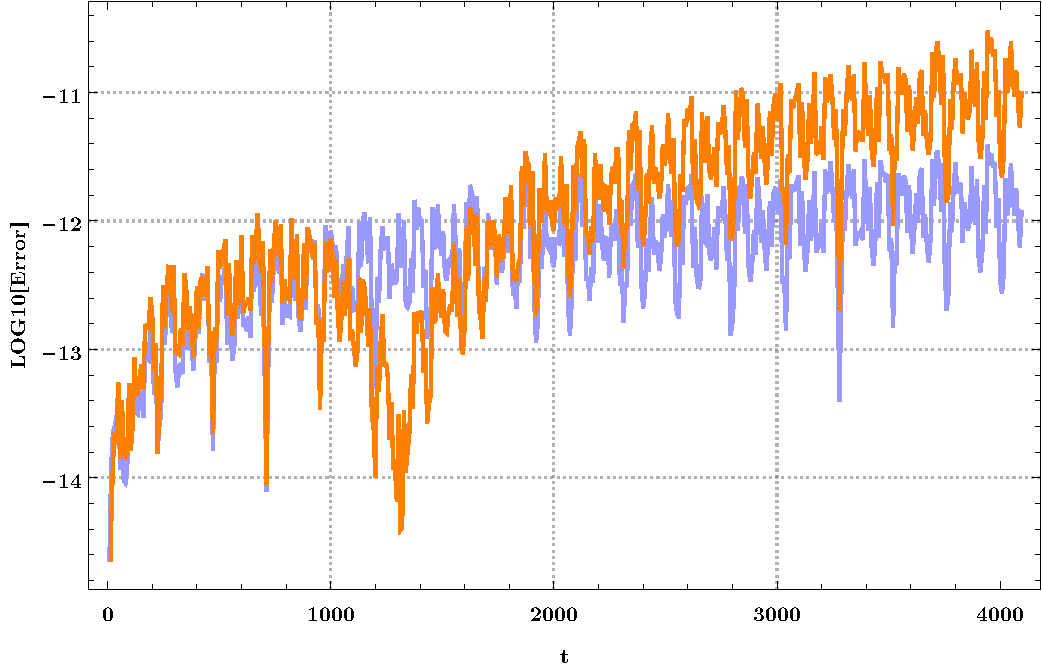
\includegraphics[width=.4\textwidth]{Fig20}}
&
\subfloat[NCDP: perturbatutako $P=1000$ integrazio]
{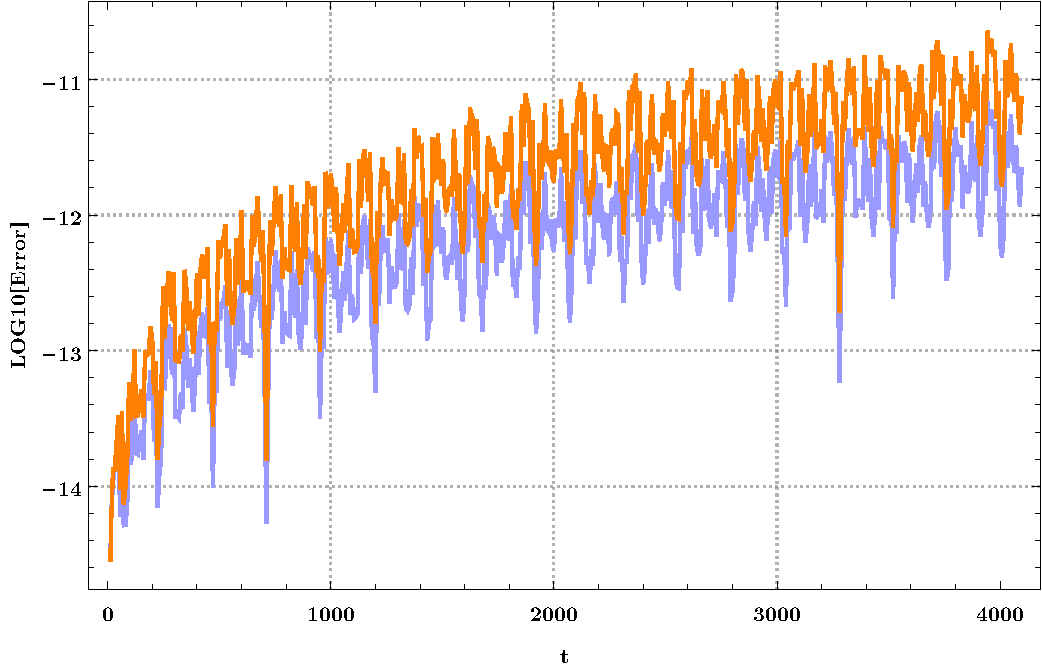
\includegraphics[width=.4\textwidth]{Fig21}}
\\
\subfloat[CDP: jatorrizko hasierako balioak]
{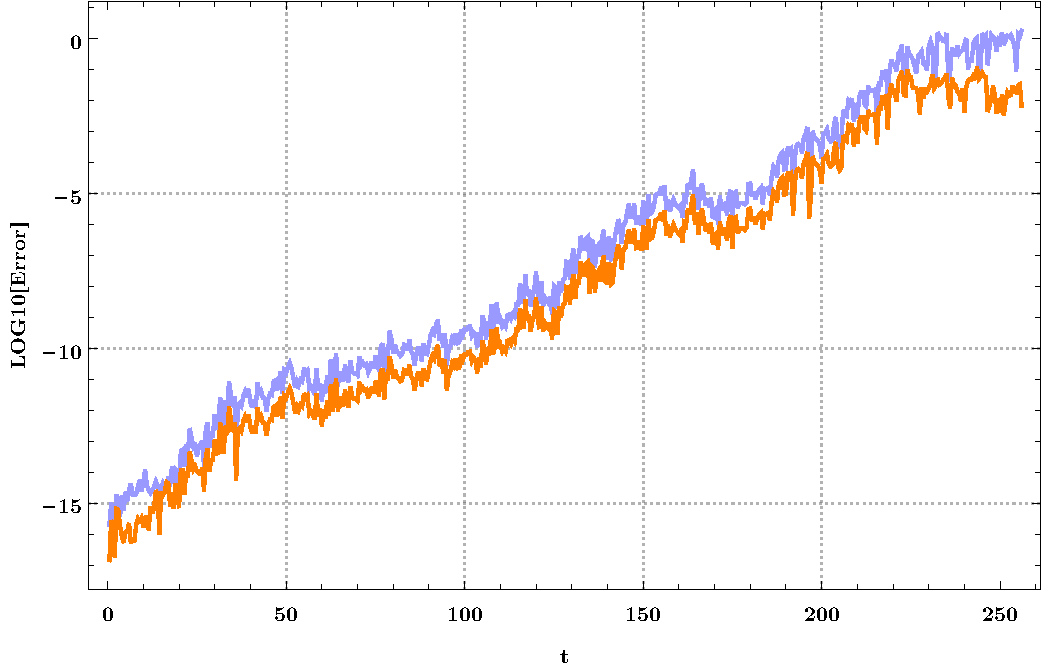
\includegraphics[width=.4\textwidth]{Fig22}}
&
\subfloat[CDP: perturbatutako $P=1000$ integrazio]
{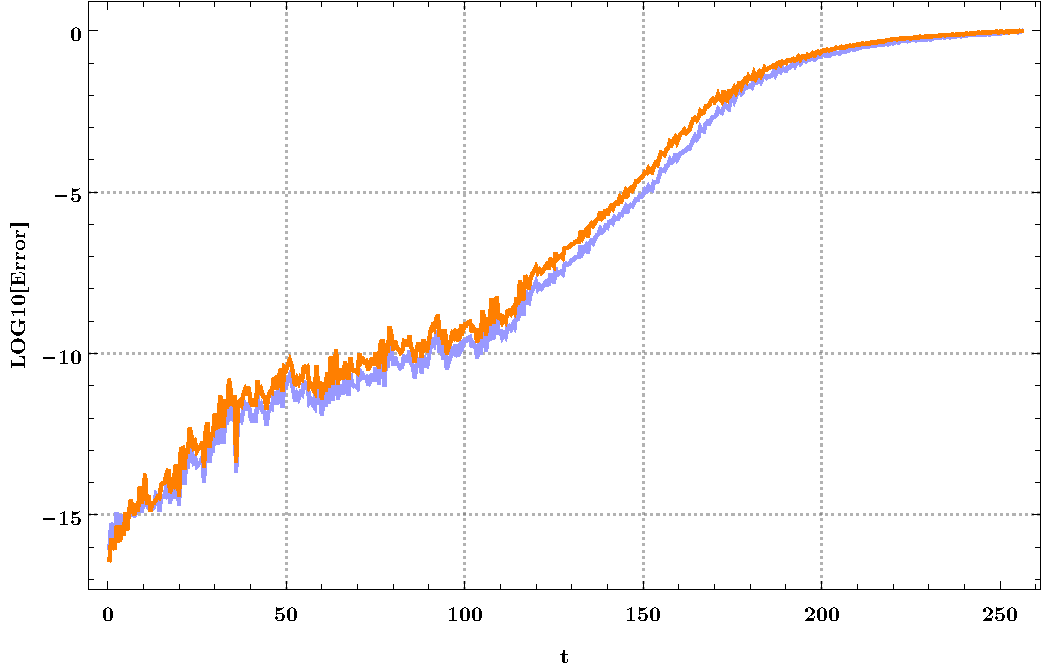
\includegraphics[width=.4\textwidth]{Fig23}}
\\
\subfloat[OSS: jatorrizko hasierako balioak]
{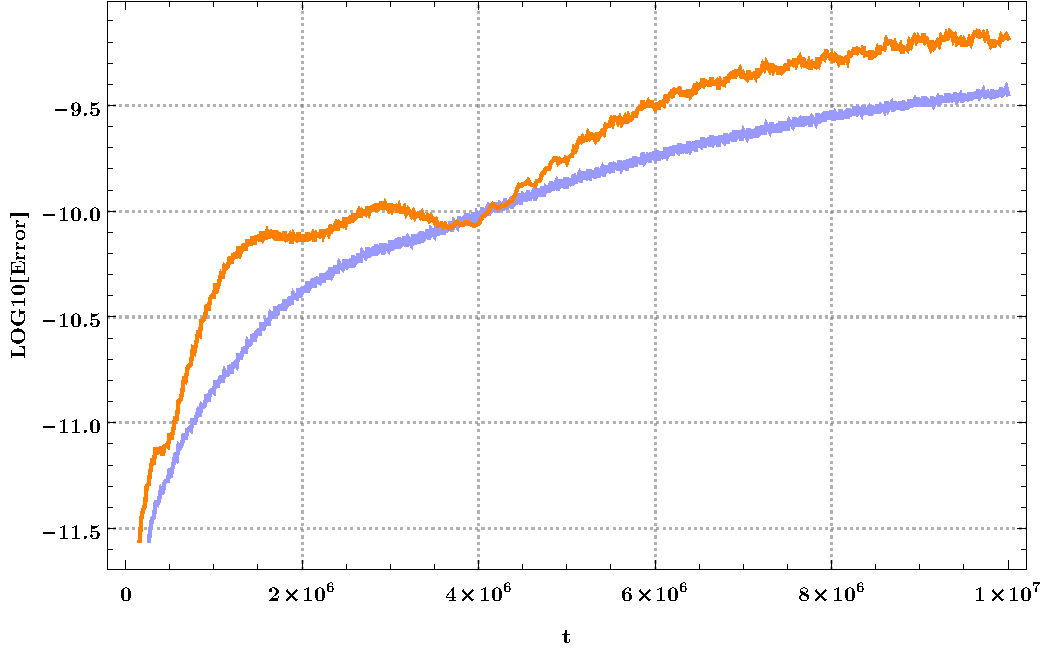
\includegraphics[width=.4\textwidth]{Fig24}}
&
\subfloat[OSS: perturbatutako $P=1000$ integrazio]
{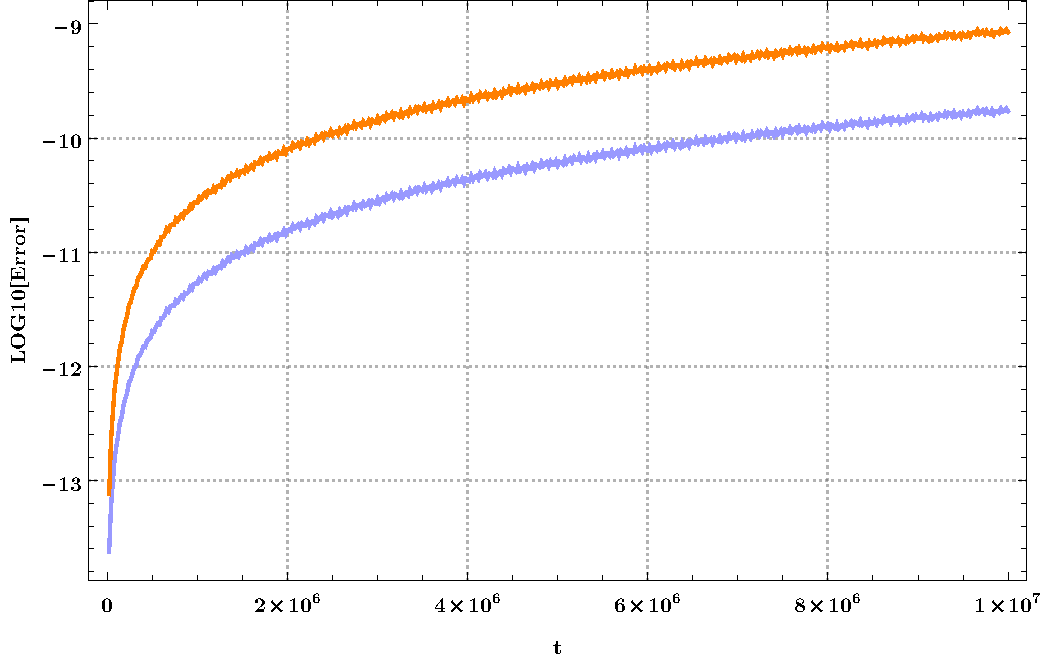
\includegraphics[width=.4\textwidth]{Fig25}}
\end{tabular}
\caption{\small Kokapen errorea (urdinez) eta kokapen errorearen estimazioa (laranjaz). Ezkerrean, perturbatu gabeko hasierako balioen integrazioak eta  eskubian, hasierako balioen perturbatutako $P=1000$ integrazioen batezbestekoak}
\label{fig:plot5}
\end{figure}


\section{Laburpena.}

Runge-Kutta metodo inplizituak (adibidez, Gauss nodoetan oinarritutako RK kolokazio metodoak) Hamiltondar sistemen doitasun altuko integrazioetarako aproposak dira. Problema ez-zurrunetarako, puntu-finkoaren iterazioan oinarritutako inplementazioa, Newton metodoaren iterazioan oinarritutako inplementazioak baino eraginkorragoa da.

Proposatutako inplementazioan, biribiltze errorearen eragina txikitzeko ahalegin berezia egin dugu eta  gainera, biribiltze errorearen estimazio kalkulatzeko aukera eman dugu. Gure inplementazioak, puntu-finkoaren iterazioan oinarritutako inplementazio onenaren birbiltze errorearen eboluzio antzekoa du eta zentzu honetan, gure inplementazioa ia optimoa da. Zenbakizko esperimentuek idei hau baieztatu dute.

Inplementazioaren gakoetako bat, puntu-finkoaren iterazioaren geratze irizpide berria da. Geratze irizpidea, beste eremu batzuetan aplikagarria izan daitekeela pentsatzen dugu.

Bestalde, puntu-finkoaren iterazioaren inplementazioaren zenbakizko esperimentu batzuetan,  energi errorearen drift lineal txiki bat ekidin ezinezkoa agertu zaigu. Energi errorearen drift-a gainditzea garrantzitsua denenerako, Newtonen iterazioan oinarritutako inplementazioa beharrezkoa izan daiteke.


